
%برای گزارشات ماهانه mscR و برای نسخه نهایی msc انتخاب شود
\documentclass[oneside,openany,msc]{AUT-Thesis}
% در این فایل، دستورها و تنظیمات مورد نیاز، آورده شده است.
%-------------------------------------------------------------------------------------------------------------------
\usepackage {indentfirst}
\usepackage{multirow}
% در ورژن جدید زی‌پرشین برای تایپ متن‌های ریاضی، این سه بسته، حتماً باید فراخوانی شود
\usepackage{amsthm,amssymb,amsmath}

\usepackage{xcolor,colortbl}
\definecolor{Gray}{gray}{0.85}

% فراخوانی بسته زی‌پرشین و تعریف قلم فارسی و انگلیسی

% بسته‌ای برای تنطیم حاشیه‌های بالا، پایین، چپ و راست صفحه
\usepackage[top=35mm, bottom=37mm, left=25mm, right=30mm]{geometry}
% بسته‌‌ای برای ظاهر شدن شکل‌ها و تصاویر متن
\usepackage{graphicx}
% بسته‌ای برای رسم کادر
\usepackage{framed} 

% بسته‌‌ای برای چاپ شدن خودکار تعداد صفحات در صفحه «معرفی پایان‌نامه»

\usepackage{lastpage}
% بسته‌ و دستوراتی برای ایجاد لینک‌های رنگی با امکان جهش
%\usepackage[pagebackref=false,colorlinks,linkcolor=blue,citecolor=blue]{hyperref}
% چنانچه قصد پرینت گرفتن نوشته خود را دارید، خط بالا را غیرفعال و  از دستور زیر استفاده کنید چون در صورت استفاده از دستور زیر‌‌، 
% لینک‌ها به رنگ سیاه ظاهر خواهند شد که برای پرینت گرفتن، مناسب‌تر است
\usepackage[pagebackref=false]{hyperref}
% بسته‌ لازم برای تنظیم سربرگ‌ها
\usepackage{fancyhdr}
%
\usepackage[toc,page]{appendix} %appendix
\usepackage{setspace}
\usepackage{algorithm}
\usepackage{algorithmic}

\usepackage{subfigure}
\usepackage[subfigure,titles]{tocloft}
\cftsetindents{figure}{0em}{3.5em}
\cftsetindents{table}{0em}{3.5em}

% CONFLICT with SUBFIGURE !
%\usepackage{subcaption}
   %\captionsetup{textfont = sl} % use slanted font shape automatically for all captions
%\usepackage[noabbrev]{cleveref}

\usepackage{caption}
\captionsetup[table]{labelsep=space}
\captionsetup[figure]{labelsep=space}
\captionsetup[table]{position=top}   %% or below




% بسته‌ای برای ظاهر شدن «مراجع» و «نمایه» در فهرست مطالب
\usepackage[nottoc,notlof,notlot]{tocbibind}


% دستورات مربوط به ایجاد نمایه
\usepackage{makeidx}
\makeindex
%%%%%%%%%%%%%%%%%%%%%%%%%%
\usepackage{backnaur}

\usepackage{longtable}
\usepackage{titlesec}

%\usepackage[Kashida=on]{xepersian}
\usepackage[perpagefootnote]{xepersian}

%\settextfont[Scale=1]{XB Niloofar}
\settextfont[Scale=0.9]{Persian Modern}
%\settextfont[Scale=1]{HM FElmi}
\setlatintextfont[Scale=0.9]{Latin Modern Roman}

%%%%%%%%%%%%%%%%%%%%%%%%%%
% چنانچه می‌خواهید اعداد در فرمول‌ها، انگلیسی باشد، خط زیر را غیرفعال کنید
\setdigitfont[Scale=0.857]{Persian Modern}
%%%%%%%%%%%%%%%%%%%%%%%%%%
% تعریف قلم‌های فارسی و انگلیسی اضافی برای استفاده در بعضی از قسمت‌های متن
\defpersianfont\titlefont[Scale=0.857]{B Titr}
% \defpersianfont\iranic[Scale=1.1]{XB Zar Oblique}%Italic}%
% \defpersianfont\nastaliq[Scale=1.2]{IranNastaliq}

%%%%%%%%%%%%%%%%%%%%%%%%%%
% دستوری برای حذف کلمه «چکیده»
\renewcommand{\abstractname}{}
% دستوری برای حذف کلمه «abstract»
%\renewcommand{\latinabstract}{}
% دستوری برای تغییر نام کلمه «اثبات» به «برهان»
\renewcommand\proofname{\textbf{برهان}}
% دستوری برای تغییر نام کلمه «کتاب‌نامه» به «مراجع»
\renewcommand{\bibname}{\hfil  مراجع}
%\renewcommand{\bibname}{\normalsize \begin{center} مراجع \end{center}}
% دستوری برای تعریف واژه‌نامه انگلیسی به فارسی
\newcommand\persiangloss[2]{#1\dotfill\lr{#2}\\}
% دستوری برای تعریف واژه‌نامه فارسی به انگلیسی 
\newcommand\englishgloss[2]{#2\dotfill\lr{#1}\\}
% تعریف دستور جدید «\پ» برای خلاصه‌نویسی جهت نوشتن عبارت «پروژه/پایان‌نامه/رساله»
\newcommand{\پ}{پروژه/پایان‌نامه/رساله }

\renewcommand\appendixname{پیوست}

%\newcommand\BackSlash{\char`\\}

%%%%%%%%%%%%%%%%%%%%%%%%%%
\SepMark{-}

% تعریف و نحوه ظاهر شدن عنوان قضیه‌ها، تعریف‌ها، مثال‌ها و ...
\theoremstyle{definition}
\newtheorem{definition}{تعریف}[section]
\newtheorem{theorem}[definition]{قضیه}
\newtheorem{lemma}[definition]{لم}
\newtheorem{proposition}[definition]{گزاره}
\newtheorem{corollary}[definition]{نتیجه}
\newtheorem{remark}[definition]{ملاحظه}
\theoremstyle{definition}
\newtheorem{example}[definition]{مثال}

%\renewcommand{\theequation}{\thechapter-\arabic{equation}}
%\def\bibname{مراجع}
\numberwithin{algorithm}{chapter}
\def\listalgorithmname{فهرست الگوریتم‌ها}
\def\listfigurename{فهرست اشکال}
\def\listtablename{فهرست جداول}

%%%%%%%%%%%%%%%%%%%%%%%%%%%%
% دستورهایی برای سفارشی کردن سربرگ صفحات
% \newcommand{\SetHeader}{
% \csname@twosidetrue\endcsname
% \pagestyle{fancy}
% \fancyhf{} 
% \fancyhead[OL,EL]{\thepage}
% \fancyhead[OR]{\small\rightmark}
% \fancyhead[ER]{\small\leftmark}
% \renewcommand{\chaptermark}[1]{%
% \markboth{\thechapter-\ #1}{}}
% }
%%%%%%%%%%%%5
%\def\MATtextbaseline{1.5}
%\renewcommand{\baselinestretch}{\MATtextbaseline}
\linespread{1.9}
%%%%%%%%%%%%%%%%%%%%%%%%%%%%%
% دستوراتی برای اضافه کردن کلمه «فصل» در فهرست مطالب

\newlength\mylenprt
\newlength\mylenchp
\newlength\mylenapp

\renewcommand\cftpartpresnum{\partname~}
\renewcommand\cftchappresnum{\chaptername~}
\renewcommand\cftchapaftersnum{}

\settowidth\mylenprt{\cftpartfont\cftpartpresnum\cftpartaftersnum}
\settowidth\mylenchp{\cftchapfont\cftchappresnum\cftchapaftersnum}
\settowidth\mylenapp{\cftchapfont\appendixname~\cftchapaftersnum}
\addtolength\mylenprt{\cftpartnumwidth}
\addtolength\mylenchp{\cftchapnumwidth}
\addtolength\mylenapp{\cftchapnumwidth}

\setlength\cftpartnumwidth{\mylenprt}
\setlength\cftchapnumwidth{\mylenchp}	

\makeatletter
{\def\thebibliography#1{\chapter*{\refname\@mkboth
   { \uppercase{\refname}}{ \uppercase{\refname}}}\list
   {[\arabic{enumi}]}{\settowidth\labelwidth{[#1]}
   \rightmargin\labelwidth
   \advance\rightmargin\labelsep
   \advance\rightmargin\bibindent
   \itemindent -\bibindent
   \listparindent \itemindent
   \parsep \z@
   \usecounter{enumi}}
   \def\newblock{}
   \sloppy
   \sfcode`\.=1000\relax}}
\makeatother

\makeatletter
\newcommand{\nextverbatimspread}[1]{%
  \def\verbatim@font{%
    \linespread{#1}\normalfont\ttfamily% Updated definition
    \gdef\verbatim@font{\normalfont\ttfamily}}% Revert to old definition
}
\makeatother

%تنظیم فاصله متن تا خط زیرنویس
\setlength{\skip\footins}{1cm}


\usepackage{booktabs}

\renewcommand{\cfttoctitlefont}{\hfil \Huge \bfseries}
\renewcommand{\cftlottitlefont}{\hfil \Huge \bfseries}
\renewcommand{\cftloftitlefont}{\hfil \Huge \bfseries}



\graphicspath{{Figures/}}
\DeclareMathOperator*{\argmin}{arg\,min}
\DeclareMathOperator*{\argmax}{arg\,max}



\setcounter{tocdepth}{2}
\setcounter{secnumdepth}{5}

\newcommand{\cchapter}[1]{\chapter[#1]{\centering #1}}

\renewcommand\thefigure{\thechapter\lr{‑}\arabic{figure}}
\renewcommand\thetable{\thechapter\lr{‑}\arabic{table}}
\renewcommand\theequation{\thechapter\lr{‑}\arabic{equation}}
\renewcommand\thesection{\thechapter\lr{‑}\arabic{section}}
\renewcommand\thesubsection{\thesection\lr{‑}\arabic{subsection}}
\renewcommand\thesubsubsection{\thesubsection\lr{‑}\arabic{subsubsection}}

\renewcommand{\labelenumi}{\arabic{enumi}- }
\renewcommand{\labelenumii}{\alph{enumii}- }
\renewcommand{\labelenumiii}{\roman{enumiii}- }
\renewcommand{\labelitemi}{$\bullet$}
\renewcommand{\labelitemii}{$\circ$}


\makeatletter
\usepackage{patchcmd}
%nkhComment: This is not working anymore:
%\patchcommand{\@makecaption}{#1: #2}{#1: #2}{}{}
\makeatother
\usepackage{multirow}
\pagestyle{fancy}

%------------------------------
\lhead{}
% Length to control the \fancyheadoffset and the calculation of \headline
% simultaneously
\newlength\FHoffset
\setlength\FHoffset{1cm}

\addtolength\headwidth{2\FHoffset}

\fancyheadoffset{\FHoffset}

% these lengths will control the headrule trimming to the left and right 
\newlength\FHleft
\newlength\FHright

% here the trimmings are controlled by the user
\setlength\FHleft{1cm}
\setlength\FHright{0cm}

% The new definition of headrule that will take into acount the trimming(s)
\newbox\FHline
\setbox\FHline=\hbox{\hsize=\paperwidth%
  \hspace*{\FHleft}%
  \rule{\dimexpr\headwidth-\FHleft-\FHright\relax}{\headrulewidth}\hspace*{\FHright}%
}
\renewcommand\headrule{\vskip-0.6\baselineskip\copy\FHline}

\renewcommand{\chaptermark}[1]{\markboth{\thechapter\lr{‑}\ #1}{}}
%\renewcommand{\headrule}{\vbox to 0pt{\hbox to\headwidth{\dotfill}\vss}}
%------------------------------
%\setdigitfont{Arial}
\newcommand*\tageq{\refstepcounter{equation}\tag{\theequation}}

\usepackage{float}
\floatstyle{plaintop}
\restylefloat{table}

\usepackage{cite}

%\usepackage{mathptmx}
\usepackage[cal=cm, bb=ams, frak=esstix, scr=esstix]{mathalfa}

\usepackage{tabularx}


%تنظیم فاصله قبل و بعد فرمول‌ها 
\setlength{\abovedisplayskip}{6pt}
\setlength{\abovedisplayshortskip}{3pt}
\setlength{\belowdisplayshortskip}{3pt}
\setlength{\belowdisplayskip}{6pt}

\renewcommand{\contentsname}{\hspace*{\fill}فهرست مطالب\hspace*{\fill}} 
\renewcommand{\listfigurename}{\hspace*{\fill}فهرست اشکال\hspace*{\fill}} 
\renewcommand{\listtablename}{\hspace*{\fill}فهرست جداول\hspace*{\fill}}


\renewcommand{\cftdotsep}{1}
\renewcommand{\cftchapleader}{\bfseries\cftdotfill{\cftsecdotsep}}% dot leaders in bold
\renewcommand{\cftchapfont}{\bfseries}
\renewcommand{\cftsecfont}{\bfseries}

 \let\origaddvspace\addvspace
 \renewcommand{\addvspace}[1]{}
 
 %\let\origappendix\appendix % save the existing appendix command
\usepackage{floatpag}

\usepackage{placeins}


%\university{دانشگاه صنعتی امیرکبیر (پلی تکنیک تهران)}
\faculty{گروه مستقل مهندسی رباتیک}

\baselineskip=2cm
\title{
تشخیص و مکان‌یابی بی‌درنگ تابلوهای راهنما و متن فارسی در ویدیوهای ترافیکی شهری
}

%برای گزارشات ماهانه به این صورت نسخه مشخص میشود
\reportVersion{چهارم}

\subject{مهندسی رباتیک}
\field{مهندسی رباتیک}


\name{نوید}
\surname{خزاعی کرقند}
\firstsupervisor{دکتر رضا صفابخش}
\thesisdate{بهمن ۱۳۹۴}

\fa-abstract{
 در سال‌های اخیر با توجه به رشد صنعت خودروهای هوشمند، چالش‌های جدیدی در درک محیط توسط خودرو یا هم‌یار راننده مطرح شده‌است. از جمله‌ی این چالش‌ها تشخیص و شناسایی علایم ترافیکی و تابلوهای راهنما در محیط است که در شرایط خاص مانند عدم کارایی سیستم‌های راه‌یابی و نقشه‌خوانی حیاتی هستند. مساله‌ی تشخیص تابلوهای راهنما به دلیل پیچیدگی بیشتر، به تازگی مورد توجه پژوهشگران قرار گرفته‌است. پیشینه‌ی پژوهش در این زمینه تنها به جاده‌های بیرون از شهر که محیط بسیار خلوت و ساده‌تری برای حل مساله دارند برمی‌گردد. از آن‌جا که هیچ مجموعه‌دادگان برچسب‌گذاری‌ شده‌ای وجود ندارد، و تنها دادگان موجود بدون برچسب نیز در محیط خارج از شهر است، در این رساله مجموعه‌دادگان جامعی از محیط شهری با بیش از صدهزار فریم تهیه شده‌است و بیش از ده هزار فریم توسط انسان برچسب‌گذاری گردیده‌است.
\textbf{ در میان پاراگراف‌ها از خط جدید (اینتر) استفاده نکنید. }
لورم ایپسوم متنی بی مفهوم است که تشکیل شده از کلمات معنی دار یا بی معنی کنار هم. کاربر با دیدن متن لورم ایپسوم تصور میکند متنی که در صفحه مشاهده میکند این متن واقعی و مربوط به توضیحات صفحه مورد نظر است واقعی است. حالا سوال اینجاست که این متن « لورم ایپسوم » به چه دردی میخورد و اساسا برای چه منظور و هدفی ساخته شده است؟ پیش از بوجود آمدن لورم ایپسوم ، طراحان وب سایت در پروژه های وب سایت و طراحان کرافیک در پروژه های طراحی کاتولوگ ، بروشور ، پوستر و ... همواره با این مشکل مواجه بودند که صفحات پروژه خود را پیش از آنکه متن اصلی توسط کارفرما ارائه گردد و در صفحه مورد نظر قرار گیرد چگونه پر کنند؟؟ اکثر طراحان با نوشتن یک جمله مانند «این یک متن نمونه است» ویا «توضیحات در این بخش قرار خواهند گرفت» و کپی آن به تعداد زیاد یک یا چند پاراگراف متن میساختند که تمامی متن ها و کلمات ، جملات و پاراگراف ها تکراری بود و از این رو منظره خوبی برای بیننده نداشت و ضمنا به هیچ وجه واقعی به نظر نمیرسید تا بتواند شکل و شمایل تمام شده پروژه را نشان دهد. 
}

\keywords{پردازش تصویر، تشخیص تابلوهای راهنما، تشخیص متن فارسی، ویدیوهای ترافیک شهری}

%%%% english
\en-abstract{
In recent years, new challenges has been raised in environment perception for autonomous vehicles and driver's assistant systems. One of the most important challenges is traffic sign and traffic panel detection which are vital navigation systems malfunction. Traffic Panel detection is recently investigated by researchers because of its higher complexity. The literature is limited to roads out of cities where there is no clutter and the problem is easy to solve.
Lorem ipsum dolor sit amet, consectetuer adipiscing elit, sed diam nonummy nibh euismod tincidunt ut laoreet dolore magna aliquam erat volutpat. Ut wisi enim ad minim veniam, quis nostrud exerci tation ullamcorper suscipit lobortis nisl ut aliquip ex ea commodo consequat. Duis autem vel eum iriure dolor in hendrerit in vulputate velit esse molestie consequat, vel illum dolore eu feugiat nulla facilisis at vero eros et accumsan et iusto odio dignissim qui blandit praesent luptatum zzril delenit augue duis dolore te feugait nulla facilisi.
\textbf{DO NOT USE NEW LINES IN ABSTARCT}
Lorem ipsum dolor sit amet, consectetuer adipiscing elit, sed diam nonummy nibh euismod tincidunt ut laoreet dolore magna aliquam erat volutpat. Ut wisi enim ad minim veniam, quis nostrud exerci tation ullamcorper suscipit lobortis nisl ut aliquip ex ea commodo consequat. Duis autem vel eum iriure dolor in hendrerit in vulputate velit esse molestie consequat, vel illum dolore eu feugiat nulla facilisis at vero eros et accumsan et iusto odio dignissim qui blandit praesent luptatum zzril delenit augue duis dolore te feugait nulla facilisi.
}
\latinkeywords{Image processing, Traffic Panel Detection, Persian Text Detection, Street Level Videos, Urban Traffic Videos, Real-time}

%\latinuniversity{Amirkabir University of Technology (Tehran Polytechnic)}
\latinfaculty{Faculty of Robotics Engineering}
\latintitle{Real-time Detection and Localization of Traffic Panels and Persian Text in Street-Level Videos}
\latinsubject{Robotics Engineering}
\latinname{\lr{Navid}}
\latinsurname{\lr{Khazaee Korghond}}
\firstlatinsupervisor{Prof. Reza Safabakhsh}
\latinthesisdate{February 2016}

\begin{document}

\pagenumbering{harfi}
\firstPage
\abstractPage
%\davaranPage
\tableofcontents \newpage
\listoffigures \newpage
\listoftables \newpage
\pagenumbering{arabic}

%You can write your chapters here to see the output, then when finished, transfer the chapter to a seperate file and include it here. While writing new chapters, you can avoid including previous ones to speed up the compile time. 

%---------------------- chap 1 ----------------------
\cchapter{مقدمه}
\pagebreak

یکی از مسایل همواره محبوب و چالش‌برانگیز در علم رباتیک، خودروهای هوشمند و هم‌یاری راننده می‌باشد. در اواخر دهه‌ی هشتاد، با ارایه‌ی اولین خودروی بدون سرنشین توسط شرکت \lr{Mercedes-Benz} که از علم بینایی ماشین استفاده می‌کرد
%\cite{benz}
، توجه پژوهشگران زیادی به مسایل گوناگون بینایی ماشین در این زمینه جلب شده‌است. 

یکی از مسایل چالش‌برانگیز در خودروهای هوشمند و نیز هم‌یاری راننده‌، تشخیص تابلوهای راهنمایی و رانندگی می‌باشد. \cite{Gonzalez2014}. در شکل
\ref{fig:signs} 
 تفاوت این دو دسته از تابلوها را مشاهده می‌کنید.


\begin{figure}[t]
\centering
    	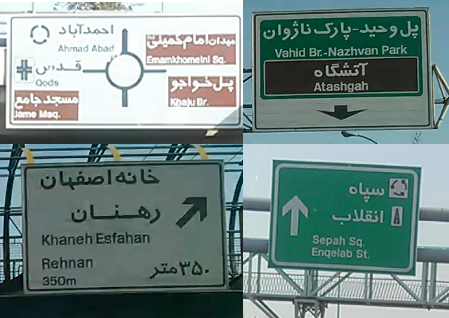
\includegraphics[height=6cm]{Figures/Panels.png}
	   	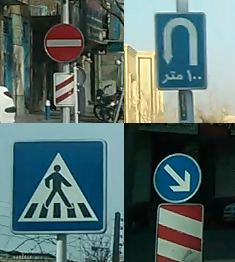
\includegraphics[height=6cm]{Figures/Signs.png}
%برای آن که کپشن تصویر در فهرست شکل‌ها به گونه دیگری بیاید:
\caption[تابلوی راهنما و علایم رانندگی]{راست: تابلوهای راهنما. چپ: علایم راهنمایی و رانندگی. }
\label{fig:signs}
\end{figure}

لورم ایپسوم ( به انگلیسی \lr{lorem ipsum} ) متنی بی مفهوم است که تشکیل شده از کلمات معنی دار یا بی معنی کنار هم. کاربر با دیدن متن لورم ایپسوم تصور میکند متنی که در صفحه مشاهده میکند این متن واقعی و مربوط به توضیحات صفحه مورد نظر است واقعی است. حالا سوال اینجاست که این متن « لورم ایپسوم » به چه دردی میخورد و اساسا برای چه منظور و هدفی ساخته شده است؟ پیش از بوجود آمدن لورم ایپسوم ، طراحان وب سایت در پروژه های وب سایت و طراحان کرافیک در پروژه های طراحی کاتولوگ ، بروشور ، پوستر و ... همواره با این مشکل مواجه بودند که صفحات پروژه خود را پیش از آنکه متن اصلی توسط کارفرما ارائه گردد و در صفحه مورد نظر قرار گیرد چگونه پر کنند؟؟ اکثر طراحان با نوشتن یک جمله مانند «این یک متن نمونه است» ویا «توضیحات در این بخش قرار خواهند گرفت» و کپی آن به تعداد زیاد یک یا چند پاراگراف متن میساختند که تمامی متن ها و کلمات ، جملات و پاراگراف ها تکراری بود و از این رو منظره خوبی برای بیننده نداشت و ضمنا به هیچ وجه واقعی به نظر نمیرسید تا بتواند شکل و شمایل تمام شده پروژه را نشان دهد. از این رو متنی ساخته شد که با دو کلمه ( به فارسی : لورم ایپسوم ) آغاز میشد وبا همین نام در بین طراحان وب و گرافیک شناخته و به سرعت محبوب شد. وب سایت های سازنده لورم ایپسوم میتوانند هر تعداد کلمه و پاراگراف که بخواهید به صوورت تکراری یا غیر تکراری برایتان بسازند و تحویلتان بدهند تا از آنها در پروژه هایتان استفاده کنید. ( لورم ایپسوم فارسی) متن های لورم ایپسوم را به زبان فارسی و علاوه بر زبان فارسی به انگلیسی ، عربی ، ترکی استانبولی و ... برایتان میسازد. زبان های دیگر نیز رفته رفته به بانک اطلاعاتی لورم ایسپوم فارسی اضافه خواهند شد.  

%--------------------- end of chap 1 ----------------
%---------------------- begin chap 2 -------------
\cchapter{پیشینه و ادبیات پژوهش}
\label{chap:lit}
\pagebreak
\section{مقدمه}

لورم ایپسوم ( به انگلیسی \lr{lorem ipsum} ) متنی بی مفهوم است که تشکیل شده از کلمات معنی دار یا بی معنی کنار هم. کاربر با دیدن متن لورم ایپسوم تصور میکند متنی که در صفحه مشاهده میکند این متن واقعی و مربوط به توضیحات صفحه مورد نظر است واقعی است. حالا سوال اینجاست که این متن « لورم ایپسوم » به چه دردی میخورد و اساسا برای چه منظور و هدفی ساخته شده است؟ پیش از بوجود آمدن لورم ایپسوم ، طراحان وب سایت در پروژه های وب سایت و طراحان کرافیک در پروژه های طراحی کاتولوگ ، بروشور ، پوستر و ... همواره با این مشکل مواجه بودند که صفحات پروژه خود را پیش از آنکه متن اصلی توسط کارفرما ارائه گردد و در صفحه مورد نظر قرار گیرد چگونه پر کنند؟؟ اکثر طراحان با نوشتن یک جمله مانند «این یک متن نمونه است» ویا «توضیحات در این بخش قرار خواهند گرفت» و کپی آن به تعداد زیاد یک یا چند پاراگراف متن میساختند که تمامی متن ها و کلمات ، جملات و پاراگراف ها تکراری بود و از این رو منظره خوبی برای بیننده نداشت و ضمنا به هیچ وجه واقعی به نظر نمیرسید تا بتواند شکل و شمایل تمام شده پروژه را نشان دهد. از این رو متنی ساخته شد که با دو کلمه ( به فارسی : لورم ایپسوم ) آغاز میشد وبا همین نام در بین طراحان وب و گرافیک شناخته و به سرعت محبوب شد. وب سایت های سازنده لورم ایپسوم میتوانند هر تعداد کلمه و پاراگراف که بخواهید به صوورت تکراری یا غیر تکراری برایتان بسازند و تحویلتان بدهند تا از آنها در پروژه هایتان استفاده کنید. ( لورم ایپسوم فارسی) متن های لورم ایپسوم را به زبان فارسی و علاوه بر زبان فارسی به انگلیسی ، عربی ، ترکی استانبولی و ... برایتان میسازد. زبان های دیگر نیز رفته رفته به بانک اطلاعاتی لورم ایسپوم فارسی اضافه خواهند شد.  

\subsection{تاریخچه}

آغاز پژوهش در این زمینه را می‌توان به وِن\LTRfootnote{ Wen} و زیلین\LTRfootnote{ Xilin} \cite{Wu2005} 
در سال ۲۰۰۵ نسبت داد که الگوریتم ارایه‌شده‌ی پیشین خود را که برای تشخیص علایم حاوی متن در محیط به‌ کار گرفته‌ شده بود \cite{Chen2004}، به صور خاص بر روی ویدیوهای شهری اعمال کرد. این پژوهش از قید عمودی بودن صفحه‌ی تابلو استفاده نمود و متن درون تابلوها را با استفاده از یک روش افزایشی\LTRfootnote{ Incremental} تشخیص داد. پس از آن در سال ۲۰۰۶ توجه بیشتری به مساله‌ی تابلوهای راهنما شد \cite{reina2006adaptive, vazquez2006approach} و علاوه بر یک روش تطبیقی\LTRfootnote{ Adaptive} برای تقطیع، شناسایی متن با استفاده از ماشین بردار پشتیبان
\LTRfootnote{ Support Vector Machine (SVM)}
نیز در آن ارایه گردید. 


در این فصل در بخش \ref{sec:panelReview} به معرفی روش‌های به کار رفته در تشخیص تابلو می‌پردازیم و ایده‌های موجود در کارهای پیشین را بررسی می‌کنیم، سپس در بخش \ref{sec:textReview} به معرفی روش‌های تشخیص متن در تابلوی راهنما می‌پردازیم. در پایان هر بخش داده‌ها و نتایج به‌دست آمده را بررسی خواهیم کرد. 

\section{تشخیص تابلوهای راهنما}
\label{sec:panelReview}

در این بخش به بررسی روش‌های موجود برای تشخیص تابلوهای راهنما پرداخته‌ایم و ایده‌های به کاررفته شده در پژوهش‌های موجود گردآوری و بررسی شده‌اند. در تشخیص تابلوی راهنما، مکان‌یابی تابلو و رفع افکنش\LTRfootnote{ Perspective} آن از اهمیت ویژه‌ای برخوردار است. قیود فیزیکی مانند مسطح بودن صفحه‌ی تابلو و یا مکان قرارگیری آن در جاده، و ویژگی‌های ظاهری مانند شکل و رنگ از جمله قیود به کار رفته در پژوهش‌های موجود هستند که در ادامه به بررسی آن‌ها در پژوهش‌های انجام‌شده می‌پردازیم. 

%---------------------- روش اول -------------
\subsection{عمودی بودن صفحه‌ی تابلوی راهنما}

در روش زیلین \cite{Wu2005}، تابلوهای راهنما طی دو مرحله استخراج می‌شوند. 

%---------------------- روش اول - ۱  -------------


\subsubsection{خوشه‌بندی نقاط با تحلیل رنگ}
ابتدا نقاط قابل تمییز\LTRfootnote{ Discriminative points } با روش شی-توماسی\LTRfootnote{ Shi-Tomasi} \cite{shi1994good}، استخراج می‌شوند. نقاطی که توسط این روش استخراج می‌شوند نقاطی خوب هستند و به آسانی تعقیب می‌شوند. در این روش ماتریس لاپلاسی برای هر نقطه در تصویر محاسبه می‌شود و مقدار ویژه‌ی کمینه‌ی $\lambda_m$ برای آن یافت می‌شود. در کل تصویر، بیشینه‌ی $\lambda_m$ یافت می‌شود و $\lambda_{max}$ نامیده می‌شود. نقاطی از تصویر که $\lambda_m$ آن‌ها بیش از 
$\% 10$ 
مقدار $\lambda_{max}$ باشد نگاه داشته می‌شوند. از این مجموعه نقاط، نقاطی که در همسایگی
 $ 3 \times 3 $ 

..........
توزیع رنگ نقاط در همسایگی هر نقطه‌ی ویژگی توسط مدل ترکیبی گاوسی\LTRfootnote{ Gaussian Mixture Model (GMM)} مدل می‌شود:
\begin{equation}
g(c) = \beta G_f(\mu_f , \theta_f) + (1 - \beta)G_b(\mu_b , \theta_b), \quad 0 \le \beta \le 1
\label{eq:GMM}
\end{equation}
که در آن $G_f$ و $G_b$ به ترتیب توزیع رنگ پیش‌زمینه و پس‌زمینه هستند. به‌این ترتیب، هر نقطه‌ی ویژگی می‌تواند با یک بردار 
$(\beta , \mu_f , \mu_b , \theta_f , \theta_b)$
که پارامترهای مدل ترکیبی گاوسی در آن نقطه‌ است نشان داده شود. وقتی اشباع رنگ\LTRfootnote{ Saturation} کم نباشد فضای رنگی اچ‌اس‌آی به دلیل مقاوت بیشتر در برابر تغییرات نوری انتخاب مناسب‌تری است که در پژوهش‌ یاد شده، مولفه‌ی اِچ آن به کار گرفته شده‌ است. با استفاده از پارامترهای مدل ترکیبی گاوسی در هر نقطه و با استفاده از روش کا-میانگین\LTRfootnote{ K-means} خوشه‌بندی انجام می‌شود و خوشه‌های
$\lbrace C_1^t , C_2^t , \dots , C_K^t \rbrace$
در زمان $t$ به‌دست می‌آیند که در پژوهش یادشده، $K$ برابر مقدار ثابت ۱۰ انتخاب شده‌است و نشان‌دهنده‌ی تعداد خوشه‌هاست. به این ترتیب، نقاطی که توزیع رنگ پس‌زمینه و پیش‌زمینه‌ی مشابه دارند در یک خوشه قرار می‌گیرند. 
$C_i^t = \left[ \ p_j^t , \dots , p_k^t \ \right] $
یک خوشه از نقطه‌ی ویژگی $j$م تا نقطه‌ی ویژگی $k$م معرفی شده‌است. پس از محاسبه‌ی یک مستطیل محدود‌کننده‌ی کمینه\LTRfootnote{ Minimu-Bounding Rectangle (MBR)}، تابلوهای راهنما در این نواحی مکان‌یابی می‌شوند. 


%---------------------- روش اول - ۲ -------------


\subsubsection{فرض عمودی بودن صفحه}

با در نظر گرفتن دو فرض زیر، با استفاده از سه نقطه یا بیشتر در دو فریم متوالی جهت تابلوی راهنما استخراج شده‌است: 
\begin{enumerate}
\item متن مورد نظر روی یک صفحه‌ی مسطح و عمودی است.
\item محور چشمی دوربین افقی می‌باشد و حرکت دوربین نیز در راستای همین محور است.
\end{enumerate}
با در نظر گرفتن سه محور مختصات برای فریم اول، فریم دوم و دوربین، و مدل کردن دوربین به صورت نقطه‌ای، اطلاعاتی در مورد صلب بودن صفحه‌ی یافت شده و عمودی بودن آن به دست می‌آید. با توجه به شکل \ref{fig:p1-worlds}، برای سه نقطه‌ی $P_2$، $P_1$ و $P_3$ در دو فریم متوالی $t_0$ و $t_1$ خواهیم داشت: 
\begin{equation}
{\left( \begin{array}{c}
x_i^{t_0} \\
y_i^{t_0} \end{array} \right) } = {f \over Z_i}
{
\left( \begin{array}{c}
X_i \\
Y_i \end{array} \right) } \quad , \quad 
{\left( \begin{array}{c}
x_i^{t_1} \\
y_i^{t_1} \end{array} \right) } = {{f} \over {Z_i - d }}
{
\left( \begin{array}{c}
X_i \\
Y_i \end{array} \right) } \quad , \ i = 1, 2, 3.
\end{equation}
که در آن $f$ فاصله کانونی دوربین است و حروف بزرگ در دستگاه مختصات دوربین و حروف کوچک در دستگاه مختصات تصویر هستند و $d$ جابه‌جایی خودرو بین دو فریم متوالی است که در عمل مقدار کوچکی است.
\begin{figure}[t]
\centering
    	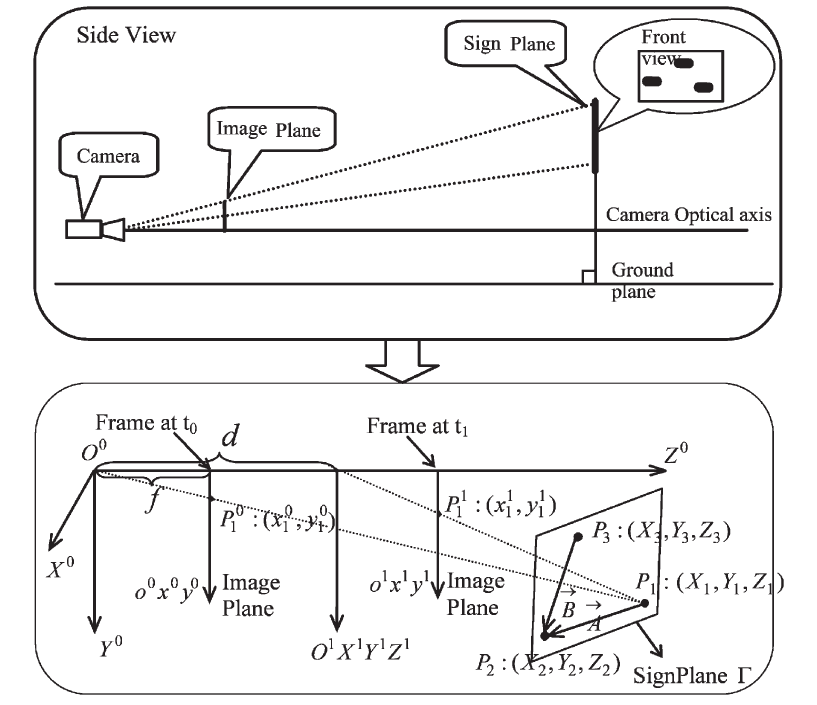
\includegraphics[width=13cm]{Figures/p1-worlds.png}
\caption[دستگاه‌های مختصات]{دستگاه‌های مختصات در نظر گرفته شده \cite{Wu2005}}
\label{fig:p1-worlds}
\end{figure}
در این پژوهش برای ارزیابی روش تشخیص، از ۲۲ ویدیوی ۳۰ ثانیه‌ای استفاده شده‌است که از روی یک خودروی در حال حرکت با سرعت‌ها و شرایط نوری متفاوت تهیه شده‌است و در مجموع دارای ۹۲ تابلوی راهنما می‌باشد. تشخیص درست 
$\% 92.4$ 
و نرخ اعلام‌های غلط 
$\% 17.7$
اعلام شده‌است. معیار درستی تشخیص همپوشانی بیش از $\% 80$ مساحت مستطیل تشخیص‌ داده‌شده و داده‌ی حقیقی زمینه‌\LTRfootnote{ Ground truth data} است. داده‌های حقیقی زمینه ابتدا توسط خود سیستم تولید شده‌اند و سپس توسط انسان به صورت دستی اصلاح شده‌اند. این داده‌ها برای تست و بررسی در دسترس نیستند.
%---------------------- روش دوم -------------
\subsection{تحلیل شکل و بازیابی جهت}

لورم ایپسوم ( به انگلیسی \lr{lorem ipsum} ) متنی بی مفهوم است که تشکیل شده از کلمات معنی دار یا بی معنی کنار هم. کاربر با دیدن متن لورم ایپسوم تصور میکند متنی که در صفحه مشاهده میکند این متن واقعی و مربوط به توضیحات صفحه مورد نظر است واقعی است. حالا سوال اینجاست که این متن « لورم ایپسوم » به چه دردی میخورد و اساسا برای چه منظور و هدفی ساخته شده است؟ پیش از بوجود آمدن لورم ایپسوم ، طراحان وب سایت در پروژه های وب سایت و طراحان کرافیک در پروژه های طراحی کاتولوگ ، بروشور ، پوستر و ... همواره با این مشکل مواجه بودند که صفحات پروژه خود را پیش از آنکه متن اصلی توسط کارفرما ارائه گردد و در صفحه مورد نظر قرار گیرد چگونه پر کنند؟؟ اکثر طراحان با نوشتن یک جمله مانند «این یک متن نمونه است» ویا «توضیحات در این بخش قرار خواهند گرفت» و کپی آن به تعداد زیاد یک یا چند پاراگراف متن میساختند که تمامی متن ها و کلمات ، جملات و پاراگراف ها تکراری بود و از این رو منظره خوبی برای بیننده نداشت و ضمنا به هیچ وجه واقعی به نظر نمیرسید تا بتواند شکل و شمایل تمام شده پروژه را نشان دهد. از این رو متنی ساخته شد که با دو کلمه ( به فارسی : لورم ایپسوم ) آغاز میشد وبا همین نام در بین طراحان وب و گرافیک شناخته و به سرعت محبوب شد. وب سایت های سازنده لورم ایپسوم میتوانند هر تعداد کلمه و پاراگراف که بخواهید به صوورت تکراری یا غیر تکراری برایتان بسازند و تحویلتان بدهند تا از آنها در پروژه هایتان استفاده کنید. ( لورم ایپسوم فارسی) متن های لورم ایپسوم را به زبان فارسی و علاوه بر زبان فارسی به انگلیسی ، عربی ، ترکی استانبولی و ... برایتان میسازد. زبان های دیگر نیز رفته رفته به بانک اطلاعاتی لورم ایسپوم فارسی اضافه خواهند شد.  
می‌کنند. 
\begin{figure}[t]
\centering
    	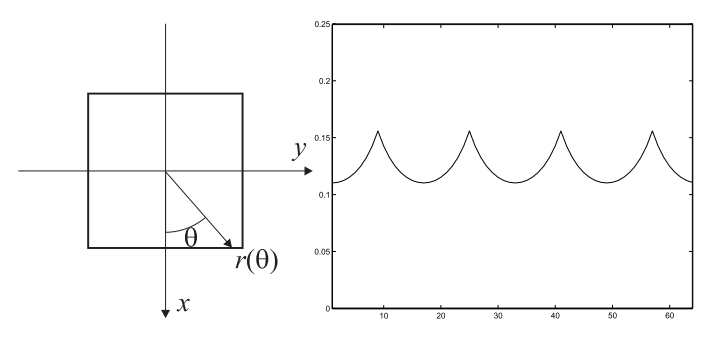
\includegraphics[width=10cm]{Figures/fft.png}
\caption[اثر (شعاعی) مستطیل]{اثر (شعاعی) مستطیل \cite{reina2006adaptive}}
\label{fig:fft}
\end{figure}
در این پژوهش، از ۶۴ نقطه روی هر لکه استفاده شده‌است که از ۰ تا $2\pi$ رادیان برای تولید اثر، شرکت داده شده‌اند. سپس مقادیر حاصل از اعمال تبدیل فوریه‌ی سریع بر روی اثر لکه با مقادیر حاصل از اعمال تبدیل فوریه‌ی سریع بر روی شکل مستطیل ایده‌آل مقایسه می‌شوند و اشکال مستطیلی به عنوان تابلو انتخاب می‌شوند. مزیت این روش مقایسه در آن است که اعمال تبدیل فوریه روی اثر شعاعی نسبت به چرخش و تغییر شکل‌های جزیی ناشی از تصویربرداری و تغییر زاویه‌ی دید مقاوم است. 
لورم ایپسوم ( به انگلیسی \lr{lorem ipsum} ) متنی بی مفهوم است که تشکیل شده از کلمات معنی دار یا بی معنی کنار هم. کاربر با دیدن متن لورم ایپسوم تصور میکند متنی که در صفحه مشاهده میکند این متن واقعی و مربوط به توضیحات صفحه مورد نظر است واقعی است. حالا سوال اینجاست که این متن « لورم ایپسوم » به چه دردی میخورد و اساسا برای چه منظور و هدفی ساخته شده است؟ پیش از بوجود آمدن لورم ایپسوم ، طراحان وب سایت در پروژه های وب سایت و طراحان کرافیک در پروژه های طراحی کاتولوگ ، بروشور ، پوستر و ... همواره با این مشکل مواجه بودند که صفحات پروژه خود را پیش از آنکه متن اصلی توسط کارفرما ارائه گردد و در صفحه مورد نظر قرار گیرد چگونه پر کنند؟؟ اکثر طراحان با نوشتن یک جمله مانند «این یک متن نمونه است» ویا «توضیحات در این بخش قرار خواهند گرفت» و کپی آن به تعداد زیاد یک یا چند پاراگراف متن میساختند که تمامی متن ها و کلمات ، جملات و پاراگراف ها تکراری بود و از این رو منظره خوبی برای بیننده نداشت و ضمنا به هیچ وجه واقعی به نظر نمیرسید تا بتواند شکل و شمایل تمام شده پروژه را نشان دهد. از این رو متنی ساخته شد که با دو کلمه ( به فارسی : لورم ایپسوم ) آغاز میشد وبا همین نام در بین طراحان وب و گرافیک شناخته و به سرعت محبوب شد. وب سایت های سازنده لورم ایپسوم میتوانند هر تعداد کلمه و پاراگراف که بخواهید به صوورت تکراری یا غیر تکراری برایتان بسازند و تحویلتان بدهند تا از آنها در پروژه هایتان استفاده کنید. ( لورم ایپسوم فارسی) متن های لورم ایپسوم را به زبان فارسی و علاوه بر زبان فارسی به انگلیسی ، عربی ، ترکی استانبولی و ... برایتان میسازد. زبان های دیگر نیز رفته رفته به بانک اطلاعاتی لورم ایسپوم فارسی اضافه خواهند شد.  
لورم ایپسوم ( به انگلیسی \lr{lorem ipsum} ) متنی بی مفهوم است که تشکیل شده از کلمات معنی دار یا بی معنی کنار هم. کاربر با دیدن متن لورم ایپسوم تصور میکند متنی که در صفحه مشاهده میکند این متن واقعی و مربوط به توضیحات صفحه مورد نظر است واقعی است. حالا سوال اینجاست که این متن « لورم ایپسوم » به چه دردی میخورد و اساسا برای چه منظور و هدفی ساخته شده است؟ پیش از بوجود آمدن لورم ایپسوم ، طراحان وب سایت در پروژه های وب سایت و طراحان کرافیک در پروژه های طراحی کاتولوگ ، بروشور ، پوستر و ... همواره با این مشکل مواجه بودند که صفحات پروژه خود را پیش از آنکه متن اصلی توسط کارفرما ارائه گردد و در صفحه مورد نظر قرار گیرد چگونه پر کنند؟؟ اکثر طراحان با نوشتن یک جمله مانند «این یک متن نمونه است» ویا «توضیحات در این بخش قرار خواهند گرفت» و کپی آن به تعداد زیاد یک یا چند پاراگراف متن میساختند که تمامی متن ها و کلمات ، جملات و پاراگراف ها تکراری بود و از این رو منظره خوبی برای بیننده نداشت و ضمنا به هیچ وجه واقعی به نظر نمیرسید تا بتواند شکل و شمایل تمام شده پروژه را نشان دهد. از این رو متنی ساخته شد که با دو کلمه ( به فارسی : لورم ایپسوم ) آغاز میشد وبا همین نام در بین طراحان وب و گرافیک شناخته و به سرعت محبوب شد. وب سایت های سازنده لورم ایپسوم میتوانند هر تعداد کلمه و پاراگراف که بخواهید به صوورت تکراری یا غیر تکراری برایتان بسازند و تحویلتان بدهند تا از آنها در پروژه هایتان استفاده کنید. ( لورم ایپسوم فارسی) متن های لورم ایپسوم را به زبان فارسی و علاوه بر زبان فارسی به انگلیسی ، عربی ، ترکی استانبولی و ... برایتان میسازد. زبان های دیگر نیز رفته رفته به بانک اطلاعاتی لورم ایسپوم فارسی اضافه خواهند شد.  

\begin{figure}[!htb]
\centering
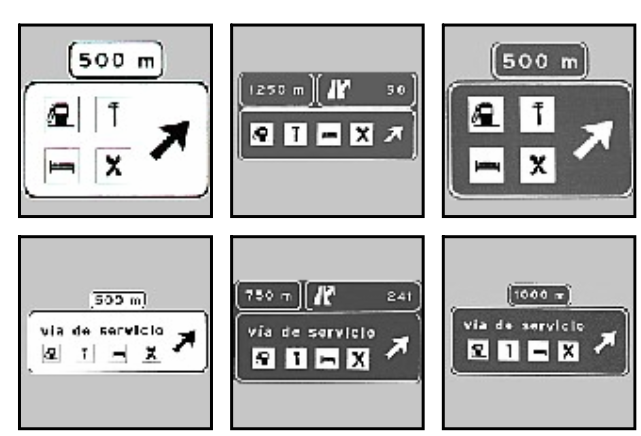
\includegraphics[width=11cm]{Figures/adaptive-types.png}
\caption[تابلوهای معرفی شده]{تابلوهای معرفی شده \cite{vazquez2006approach}.
به ترتیب از چپ به راست و از بالا به پایین:
 \lr{S-266a S-266, S-264, S-263a, S-263, S-261}
}
\label{fig:adaptive-types}
\end{figure}

\begin{table}[!htb]
\begin{center}
\def\arraystretch{2.5}
\begin{tabular}{|c|c|c|c|c|c|c|}
\hline
نوع دسته & 
\lr{S-266a} & \lr{S-266}  & \lr{S-264} & \lr{S-263a} & \lr{S-263} & \lr{S-261}\\
\hline
دقت تشخیص & 
$\% 83.19 $ & $\% 77.78 $ & $\% 75.00 $  & $\% 86.67 $ & $\% 82.35 $ & $\% 78.00$ \\
\hline
دقت دسته‌بندی & 
$\% 83.19 $ & $\% 77.78 $ & $\% 75.00 $  & $\% 86.67$ & $ \%82.35 $ & $\% 78.00 $ \\
\hline
\end{tabular}
\caption[درصد تشخیص درست]{درصد تشخیص درست دسته‌های معرفی شده \cite{vazquez2006approach}}
\label{tab:adaptive}
\end{center}
\end{table}
لورم ایپسوم ( به انگلیسی \lr{lorem ipsum} ) متنی بی مفهوم است که تشکیل شده از کلمات معنی دار یا بی معنی کنار هم. کاربر با دیدن متن لورم ایپسوم تصور میکند متنی که در صفحه مشاهده میکند این متن واقعی و مربوط به توضیحات صفحه مورد نظر است واقعی است. حالا سوال اینجاست که این متن « لورم ایپسوم » به چه دردی میخورد و اساسا برای چه منظور و هدفی ساخته شده است؟ پیش از بوجود آمدن لورم ایپسوم ، طراحان وب سایت در پروژه های وب سایت و طراحان کرافیک در پروژه های طراحی کاتولوگ ، بروشور ، پوستر و ... همواره با این مشکل مواجه بودند که صفحات پروژه خود را پیش از آنکه متن اصلی توسط کارفرما ارائه گردد و در صفحه مورد نظر قرار گیرد چگونه پر کنند؟؟ اکثر طراحان با نوشتن یک جمله مانند «این یک متن نمونه است» ویا «توضیحات در این بخش قرار خواهند گرفت» و کپی آن به تعداد زیاد یک یا چند پاراگراف متن میساختند که تمامی متن ها و کلمات ، جملات و پاراگراف ها تکراری بود و از این رو منظره خوبی برای بیننده نداشت و ضمنا به هیچ وجه واقعی به نظر نمیرسید تا بتواند شکل و شمایل تمام شده پروژه را نشان دهد. از این رو متنی ساخته شد که با دو کلمه ( به فارسی : لورم ایپسوم ) آغاز میشد وبا همین نام در بین طراحان وب و گرافیک شناخته و به سرعت محبوب شد. وب سایت های سازنده لورم ایپسوم میتوانند هر تعداد کلمه و پاراگراف که بخواهید به صوورت تکراری یا غیر تکراری برایتان بسازند و تحویلتان بدهند تا از آنها در پروژه هایتان استفاده کنید. ( لورم ایپسوم فارسی) متن های لورم ایپسوم را به زبان فارسی و علاوه بر زبان فارسی به انگلیسی ، عربی ، ترکی استانبولی و ... برایتان میسازد. زبان های دیگر نیز رفته رفته به بانک اطلاعاتی لورم ایسپوم فارسی اضافه خواهند شد.  
%---------------------- روش سوم -------------
\subsection{استفاده از ویژگی‌های ظاهری و مدل کیسه کلمات بینایی}
\label{subsec:gonzalez}

 از یک لبه‌یاب کنی اصلاح شده استفاده شده‌است. دو اصلاح انجام شده بر روی این لبه‌یاب، یکی استفاده از هسته‌ی زیر برای افزایش تضاد لبه‌ها است: 
\begin{equation}
\begin{bmatrix} 0 & -1 & 0 \\ -1 & 5 & -1 \\ 0 & -1 & 0 \end{bmatrix}
\end{equation}

زاویه‌ی چرخش 
$\alpha$
 تابلو در نظر گرفته می‌شود. به این ترتیب یک ماتریس چرخش براتبدیل نقاط $x$ و $y$ تابلو ساخته می‌شود:
 
\begin{equation}
\begin{bmatrix} \cos \alpha & \sin \alpha & (1-\cos \alpha) x_0 - \sin \alpha \cdot y_0 \\
-\sin \alpha & \cos \alpha &  \sin \alpha \cdot x_0 + (1-\cos \alpha) y_0
\end{bmatrix}
\end{equation}
برای تشخیص نواحی آبی‌رنگ، از \lr{AND} منطقی سه روش زیر استفاده شده‌است: 
\begin{itemize}
\item{آستانه‌ی رنگ قرمز}:
مقدار مولفه‌ی آر در فضای آرجی‌بی کمتر از حد آستانه‌ای ۹۰ باشد.
\item{آستانه‌ی رنگ آبی}:
محدوده‌ی مولفه‌ی اچ در فضای اچ‌اس‌وی\LTRfootnote{ HSV} بین مقادیر آستانه‌ای ۲۰۰ و ۲۸۰ درجه باشد. 
\item{روش اوتسو\LTRfootnote{ Otsu} \cite{otsu1975threshold} بر روی تفاضل مولفه‌ی قرمز و آبی}:
در این روش تصویر حاصل از قدر مطلق تفاضل مولفه‌ی قرمز و آبی به الگوریتم اوتسو داده‌ شده‌است. این الگوریتم برای دودویی کردن تصاویر به کار می‌رود، به شکلی که حد آستانه‌ی مناسبی برای آستانه‌ای کردن تصویر می‌یابد که در آن آستانه، واریانس درون دو دسته‌ی ایجاد شده (برای مثال، پس‌زمینه و پیش‌زمینه) کمینه باشد.
\end{itemize}
برای تشخیص نواحی سفیدرنگ، از روش نواحی حدی بیشینه پایدار استفاده شده‌است که به کمک آن می‌توان نواحی روشن روی نواحی تیره را تشخیص داد و پیشتر توضیح داده‌شد. 

در شکل‌های \ref{fig:bluep5} و \ref{fig:withep5} نتایج این دو آستانه‌ای کردن را مشاهده می‌کنید.
\begin{figure}[h]
\centering
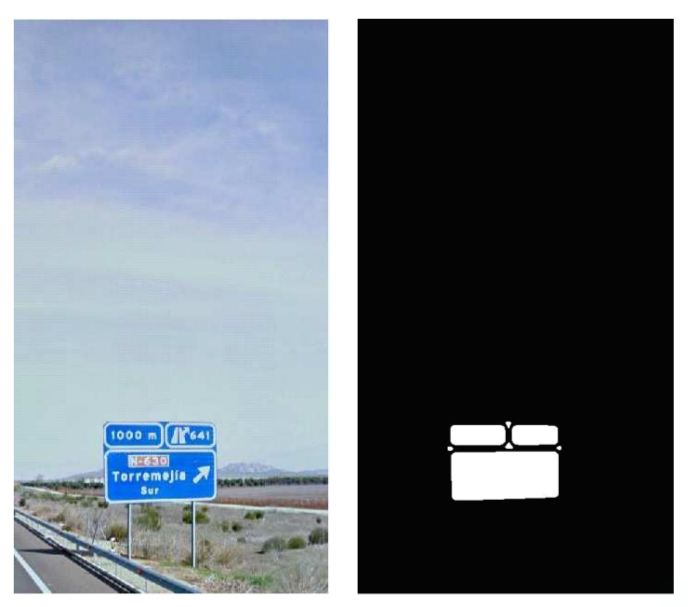
\includegraphics[width=7cm]{Figures/bluepp5.png}
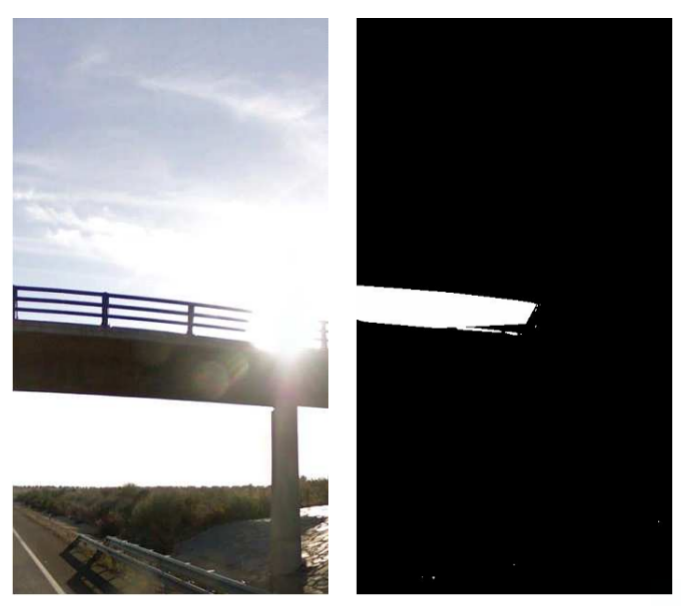
\includegraphics[width=7cm]{Figures/blue-fp5.png}
\caption[آستانه‌ای سازی رنگ آبی]{آستانه‌ای سازی رنگ آبی \cite{gonzalez2013traffic} (راست نمونه‌ی مثبت و چپ نمونه‌ی منفی)}
\label{fig:bluep5}
\end{figure}
\begin{figure}[h]
\centering
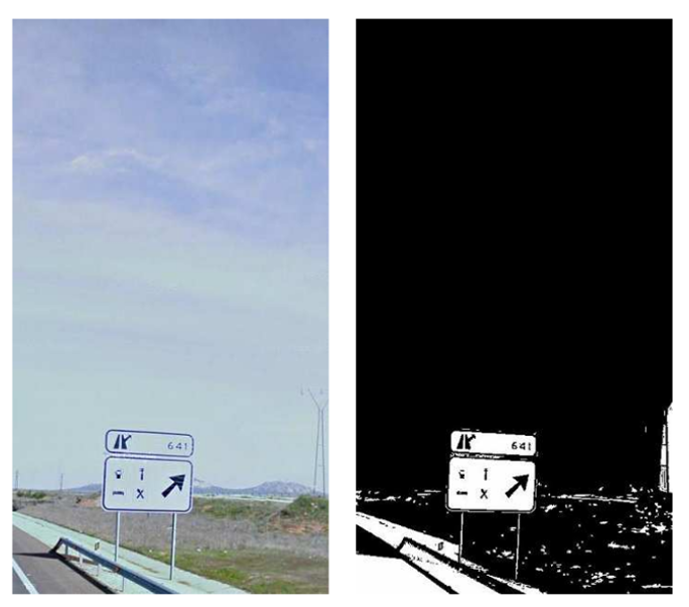
\includegraphics[width=7cm]{Figures/withe-pp5.png}
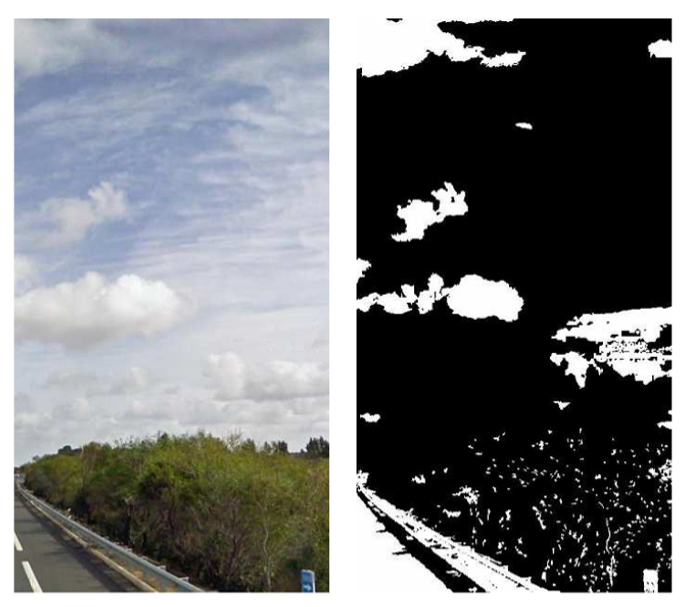
\includegraphics[width=7cm]{Figures/withe-fp5.png}
\caption[آستانه‌ای سازی رنگ سفید]{آستانه‌ای سازی رنگ سفید \cite{gonzalez2013traffic} (راست نمونه‌ی مثبت و چپ نمونه‌ی منفی)}
\label{fig:withep5}
\end{figure}

 بهترین نتایج با توصیف‌گر هیستوگرام دگرگون‌شده‌ی رنگ در جدول \ref{tab:tch} آورده شده‌است. 
\begin{table}[h]
\begin{center}
\def\arraystretch{2}
\begin{tabular}{|c|c|c|c|c|}
\hline
نوع دسته & 
نرخ تشخیص & حساسیت & تشخیص & معیار اِف \\
\hline

بالای جاده & 
$\% 98.70$ & $0.8821$ & $0.8817$ & $0.8819$ \\
\hline

کنار جاده & 
$\% 98.15$ & $0.7464$ & $0.4772$ & $0.6118$ \\
\hline
\end{tabular}
\caption[ارزیابی با توصیف‌گر هیستوگرام دگرگون‌شده‌ی رنگ]{ارزیابی با توصیف‌گر هیستوگرام دگرگون‌شده‌ی رنگ \cite{gonzalez2013traffic}}
\label{tab:tch}
\end{center}
\end{table}
%-----------------‌----- روش چهارم -------------
\subsection{اطلاعات ساختاری و زمانی}

دقت\LTRfootnote{ Precision}، یادآوری\LTRfootnote{ Recall} و معیار اِف به ترتیب در فرمول‌های \eqref{eq:precision}، \eqref{eq:recall} و \eqref{eq:fmeasure} آورده شده‌اند.
\begin{equation}
{\text{دقت}}  = { {TP} \over {TP + FP}}
\label{eq:precision}
\end{equation}
\begin{equation}
{\text{یادآوری}}  = { {TP} \over {TP + FN}}
\label{eq:recall}
\end{equation}
\begin{equation}
{\text{معیار اِف}}  = 2 * { {\text{دقت}*\text{یادآوری}} \over {\text{دقت}+\text{یادآوری}}}
\label{eq:fmeasure}
\end{equation}
 ارزیابی این پژوهش روی این پایگاه داده در مقایسه با روش‌های دیگر در جدول \ref{tab:mirmehdi} آورده شده‌است. 
\begin{table}[h]
\begin{center}
\def\arraystretch{2}
\begin{tabular}{|c|c|c|c|c|}
\hline
پژوهش & 
دقت & یادآوری & معیار اِف \\
\hline

رینا و همکاران \cite{reina2006adaptive} & 
$0.58$ & $0.64$ & $0.61$  \\
\hline

گنزالز و همکاران \cite{gonzalez2012text} & 
$0.54$ & $0.68$ & $0.60$  \\
\hline
میرمهدی و همکاران \cite{Greenhalgh2015} & 
$0.96$ & $0.90$ & $0.93$  \\
\hline
\end{tabular}
\caption[ارزیابی انجام‌شده در روش گنزالز]{ارزیابی انجام‌شده در\cite{gonzalez2013traffic}}
\label{tab:mirmehdi}
\end{center}
\end{table}
%-----------------‌----- پایان تشخیص تابلو -------------
\section{تشخیص متن در تابلوی راهنما}
\label{sec:textReview}
پس از استخراج تابلوهای راهنما، جست‌وجو به دنبال متن درون آن آغاز می‌گردد.
\subsection{روش‌های مبتنی بر لبه}

لورم ایپسوم ( به انگلیسی \lr{lorem ipsum} ) متنی بی مفهوم است که تشکیل شده از کلمات معنی دار یا بی معنی کنار هم. کاربر با دیدن متن لورم ایپسوم تصور میکند متنی که در صفحه مشاهده میکند این متن واقعی و مربوط به توضیحات صفحه مورد نظر است واقعی است. حالا سوال اینجاست که این متن « لورم ایپسوم » به چه دردی میخورد و اساسا برای چه منظور و هدفی ساخته شده است؟ پیش از بوجود آمدن لورم ایپسوم ، طراحان وب سایت در پروژه های وب سایت و طراحان کرافیک در پروژه های طراحی کاتولوگ ، بروشور ، پوستر و ... همواره با این مشکل مواجه بودند که صفحات پروژه خود را پیش از آنکه متن اصلی توسط کارفرما ارائه گردد و در صفحه مورد نظر قرار گیرد چگونه پر کنند؟؟ اکثر طراحان با نوشتن یک جمله مانند «این یک متن نمونه است» ویا «توضیحات در این بخش قرار خواهند گرفت» و کپی آن به تعداد زیاد یک یا چند پاراگراف متن میساختند که تمامی متن ها و کلمات ، جملات و پاراگراف ها تکراری بود و از این رو منظره خوبی برای بیننده نداشت و ضمنا به هیچ وجه واقعی به نظر نمیرسید تا بتواند شکل و شمایل تمام شده پروژه را نشان دهد. از این رو متنی ساخته شد که با دو کلمه ( به فارسی : لورم ایپسوم ) آغاز میشد وبا همین نام در بین طراحان وب و گرافیک شناخته و به سرعت محبوب شد. وب سایت های سازنده لورم ایپسوم میتوانند هر تعداد کلمه و پاراگراف که بخواهید به صوورت تکراری یا غیر تکراری برایتان بسازند و تحویلتان بدهند تا از آنها در پروژه هایتان استفاده کنید. ( لورم ایپسوم فارسی) متن های لورم ایپسوم را به زبان فارسی و علاوه بر زبان فارسی به انگلیسی ، عربی ، ترکی استانبولی و ... برایتان میسازد. زبان های دیگر نیز رفته رفته به بانک اطلاعاتی لورم ایسپوم فارسی اضافه خواهند شد.  
%-------------- رنگ
%---------------- چینش متن

\subsection{تقطیع تطبیقی}
لورم ایپسوم ( به انگلیسی \lr{lorem ipsum} ) متنی بی مفهوم است که تشکیل شده از کلمات معنی دار یا بی معنی کنار هم. کاربر با دیدن متن لورم ایپسوم تصور میکند متنی که در صفحه مشاهده میکند این متن واقعی و مربوط به توضیحات صفحه مورد نظر است واقعی است. حالا سوال اینجاست که این متن « لورم ایپسوم » به چه دردی میخورد و اساسا برای چه منظور و هدفی ساخته شده است؟ پیش از بوجود آمدن لورم ایپسوم ، طراحان وب سایت در پروژه های وب سایت و طراحان کرافیک در پروژه های طراحی کاتولوگ ، بروشور ، پوستر و ... همواره با این مشکل مواجه بودند که صفحات پروژه خود را پیش از آنکه متن اصلی توسط کارفرما ارائه گردد و در صفحه مورد نظر قرار گیرد چگونه پر کنند؟؟ اکثر طراحان با نوشتن یک جمله مانند «این یک متن نمونه است» ویا «توضیحات در این بخش قرار خواهند گرفت» و کپی آن به تعداد زیاد یک یا چند پاراگراف متن میساختند که تمامی متن ها و کلمات ، جملات و پاراگراف ها تکراری بود و از این رو منظره خوبی برای بیننده نداشت و ضمنا به هیچ وجه واقعی به نظر نمیرسید تا بتواند شکل و شمایل تمام شده پروژه را نشان دهد. از این رو متنی ساخته شد که با دو کلمه ( به فارسی : لورم ایپسوم ) آغاز میشد وبا همین نام در بین طراحان وب و گرافیک شناخته و به سرعت محبوب شد. وب سایت های سازنده لورم ایپسوم میتوانند هر تعداد کلمه و پاراگراف که بخواهید به صوورت تکراری یا غیر تکراری برایتان بسازند و تحویلتان بدهند تا از آنها در پروژه هایتان استفاده کنید. ( لورم ایپسوم فارسی) متن های لورم ایپسوم را به زبان فارسی و علاوه بر زبان فارسی به انگلیسی ، عربی ، ترکی استانبولی و ... برایتان میسازد. زبان های دیگر نیز رفته رفته به بانک اطلاعاتی لورم ایسپوم فارسی اضافه خواهند شد.  

 
\begin{table}[h]
\begin{center}
\def\arraystretch{2}
\begin{tabular}{|c|c|c|c|c|c|}
\hline
 خطوط متن (\lr{T}) & خطوط متن (\lr{F}) & اجزا (\lr{T}) & اجزا (\lr{F}) & کلمات (\lr{T}) & کلمات (\lr{F}) \\
\hline
 $98.56$ & $0.56$ & $96.64$ & $1.72$ & $84.35$ & $3.15$ \\
\hline
\end{tabular}
\caption[نرخ تشخیص روش گنزالز]{درصد نرخ تشخیص روش گنزالز \cite{Gonzalez2009}}
\label{tab:n1text}
\end{center}
\end{table}
\begin{center}
\begin{figure}[h]
\centering
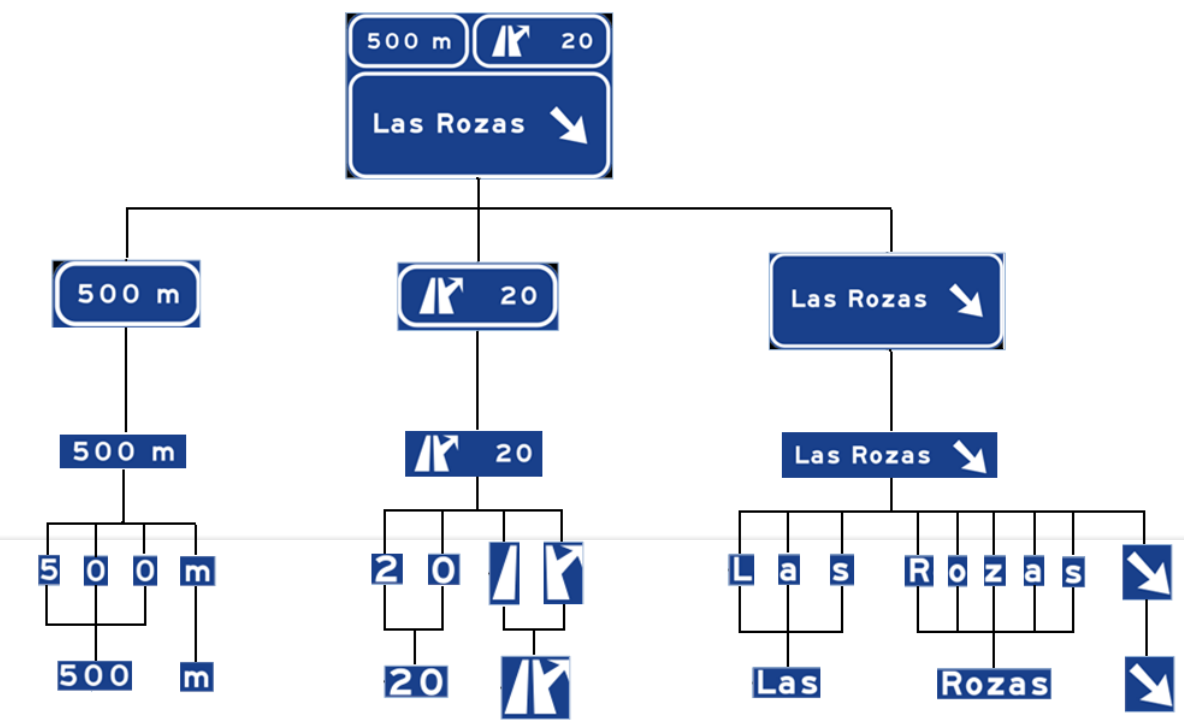
\includegraphics[width=14cm]{n1hir.png}
\caption[سلسله‌مراتب در روش گنزالز]{سلسله‌مراتب در روش گنزالز \cite{Gonzalez2009}. به ترتیب از بالا به پایین: تابلو، قاب‌های اطلاعاتی، خطوط، اجزا و حروف، کلمات.}
\label{fig:n1hir}
\end{figure}
\end{center}

\subsection{اجزای متصل و نواحی حدی بیشینه پایدار}
لورم ایپسوم ( به انگلیسی \lr{lorem ipsum} ) متنی بی مفهوم است که تشکیل شده از کلمات معنی دار یا بی معنی کنار هم. کاربر با دیدن متن لورم ایپسوم تصور میکند متنی که در صفحه مشاهده میکند این متن واقعی و مربوط به توضیحات صفحه مورد نظر است واقعی است. حالا سوال اینجاست که این متن « لورم ایپسوم » به چه دردی میخورد و اساسا برای چه منظور و هدفی ساخته شده است؟ پیش از بوجود آمدن لورم ایپسوم ، طراحان وب سایت در پروژه های وب سایت و طراحان کرافیک در پروژه های طراحی کاتولوگ ، بروشور ، پوستر و ... همواره با این مشکل مواجه بودند که صفحات پروژه خود را پیش از آنکه متن اصلی توسط کارفرما ارائه گردد و در صفحه مورد نظر قرار گیرد چگونه پر کنند؟؟ اکثر طراحان با نوشتن یک جمله مانند «این یک متن نمونه است» ویا «توضیحات در این بخش قرار خواهند گرفت» و کپی آن به تعداد زیاد یک یا چند پاراگراف متن میساختند که تمامی متن ها و کلمات ، جملات و پاراگراف ها تکراری بود و از این رو منظره خوبی برای بیننده نداشت و ضمنا به هیچ وجه واقعی به نظر نمیرسید تا بتواند شکل و شمایل تمام شده پروژه را نشان دهد. از این رو متنی ساخته شد که با دو کلمه ( به فارسی : لورم ایپسوم ) آغاز میشد وبا همین نام در بین طراحان وب و گرافیک شناخته و به سرعت محبوب شد. وب سایت های سازنده لورم ایپسوم میتوانند هر تعداد کلمه و پاراگراف که بخواهید به صوورت تکراری یا غیر تکراری برایتان بسازند و تحویلتان بدهند تا از آنها در پروژه هایتان استفاده کنید. ( لورم ایپسوم فارسی) متن های لورم ایپسوم را به زبان فارسی و علاوه بر زبان فارسی به انگلیسی ، عربی ، ترکی استانبولی و ... برایتان میسازد. زبان های دیگر نیز رفته رفته به بانک اطلاعاتی لورم ایسپوم فارسی اضافه خواهند شد.  

\section{جمع‌بندی}
تمامی پژوهش‌های پیشین به جز تعداد اندکی، تمرکز حل مساله را بر روی شرایط ساده‌تر بیرون از شهر گذاشته‌اند که شامل برترین پژوهش‌ها، میرمهدی و گنزالز می‌شوند. هیچ‌یک از پژوهش‌ها جز مورد میرمهدی مجموعه دادگان را در اختیار قرار نداده‌اند که آن هم فاقد برچسب‌گذاری است. رنگ سفید تنها در پژوهش گنزالز در مورد جاده‌های بیرون شهر به صورت جدی اثر داده شده‌است. تنها مورد موفق در محیط شهری نیز به بررسی رنگ آبی بسنده کرده‌است. دقت بالای این پژوهش‌ها ناشی از حل مساله در شرایط مهندسی‌شده و غیر واقعی بوده است. 
%---------------------- end chap 2 -------------

%------------------------ Start chapter 3 -------------
\cchapter{روش حل مساله}
\pagebreak

\section{مقدمه}
 
با توجه به کارهای پیشین، مشاهده می‌کنیم که حل مساله با شرایط خاص در جاده و محیط خلوت انجام شده‌است. در این روش‌ها تعداد رنگ‌ها نیز محدود بوده‌است و در پژوهش‌های برتر، رنگ سفید حذف شده‌است، چرا که دشواری مساله را چندین برابر می‌کند. در این رساله، برای اولین بار مساله‌ی تشخیص تابلوهای راهنما و متن آن را در محیط شهری و شلوغ تعریف می‌کنیم. با توجه به این که چنین مجموعه‌ دادگانی به صورت استاندارد وجود ندارد، مجموعه دادگان تهیه و استانداردسازی شده‌است که در فصل بعد به معرفی آن خواهیم پرداخت. سپس در ادامه گام‌های مورد نیاز برای تشخیص تابلو و تشخیص متن فارسی در آن آورده می‌شود \cite{khazaee2016aut}. 


\section{ویژگی‌های تابلوها}
\label{subsec:panelattr}لورم ایپسوم ( به انگلیسی \lr{lorem ipsum} ) متنی بی مفهوم است که تشکیل شده از کلمات معنی دار یا بی معنی کنار هم. کاربر با دیدن متن لورم ایپسوم تصور میکند متنی که در صفحه مشاهده میکند این متن واقعی و مربوط به توضیحات صفحه مورد نظر است واقعی است. حالا سوال اینجاست که این متن « لورم ایپسوم » به چه دردی میخورد و اساسا برای چه منظور و هدفی ساخته شده است؟ پیش از بوجود آمدن لورم ایپسوم ، طراحان وب سایت در پروژه های وب سایت و طراحان کرافیک در پروژه های طراحی کاتولوگ ، بروشور ، پوستر و ... همواره با این مشکل مواجه بودند که صفحات پروژه خود را پیش از آنکه متن اصلی توسط کارفرما ارائه گردد و در صفحه مورد نظر قرار گیرد چگونه پر کنند؟؟ اکثر طراحان با نوشتن یک جمله مانند «این یک متن نمونه است» ویا «توضیحات در این بخش قرار خواهند گرفت» و کپی آن به تعداد زیاد یک یا چند پاراگراف متن میساختند که تمامی متن ها و کلمات ، جملات و پاراگراف ها تکراری بود و از این رو منظره خوبی برای بیننده نداشت و ضمنا به هیچ وجه واقعی به نظر نمیرسید تا بتواند شکل و شمایل تمام شده پروژه را نشان دهد. از این رو متنی ساخته شد که با دو کلمه ( به فارسی : لورم ایپسوم ) آغاز میشد وبا همین نام در بین طراحان وب و گرافیک شناخته و به سرعت محبوب شد. وب سایت های سازنده لورم ایپسوم میتوانند هر تعداد کلمه و پاراگراف که بخواهید به صوورت تکراری یا غیر تکراری برایتان بسازند و تحویلتان بدهند تا از آنها در پروژه هایتان استفاده کنید. ( لورم ایپسوم فارسی) متن های لورم ایپسوم را به زبان فارسی و علاوه بر زبان فارسی به انگلیسی ، عربی ، ترکی استانبولی و ... برایتان میسازد. زبان های دیگر نیز رفته رفته به بانک اطلاعاتی لورم ایسپوم فارسی اضافه خواهند شد.  


\begin{itemize}
\renewcommand{\labelitemii}{$\circ$}

\item مستطیل معمول (\lr{NR})\LTRfootnote{ Normal Rectangle}: 

در این دسته تنها یک قاب در تابلو مشاهده می‌شود. اگر درون تابلو ناحیه‌ی مستطیل شکل با رنگ دیگر ولی بدون قاب جدا کننده وجود داشته باشد، باز هم تابلو از این دسته خواهد بود. یک نمونه در شکل \ref{fig:NR} آورده‌ شده‌است.

\item چند مستطیلی (\lr{MR})\LTRfootnote{ Multiple Rectangles}: 

تابلو در این دسته می‌تواند چندین قاب مستطیلی را در خود جای‌ دهد. این حالت «می‌تواند» در برخی از تابلوهای دارای چند پس‌زمینه رخ می‌دهد. همچنین ممکن است در تابلو با تنها با یک پس‌زمینه، برای تاکید رخ دهد. حالت دیگر، زمانی رخ می‌دهد که چندین تابلوی مستطیل شکل افقی روی هم‌دیگر قرار گرفته باشند. این تابلوها در مجموعه‌دادگان یک تابلو در نظر گرفته شده‌اند و نمونه‌ای از آن‌ را در شکل \ref{fig:MR} مشاهده می‌کنید. 

\item پنج ضلعی (\lr{BP/TP})\LTRfootnote{ Big/Tiny Pentagon}: 

این تابلوها شکل پنج ضلعی دارند که به شکل معمول سر پنج ضلعی به چپ یا راست اشاره می‌کند. این تابلوها به دو شکل بزرگ و کوچک (لاغر) موجود هستند که نمونه‌ی کوچک معمول‌تر است و تفاوت آن با نسخه‌ی بزگ در کشیدگی، پهنای کمتر و در نتیجه بسته‌تر بودن زاویه‌ی علامت پیکان‌مانند آن در سر پنج ضلعی می‌باشد. یک نمونه تابلوی پنج ضلعی بزرگ در شکل \ref{fig:BP} آورده شده‌است. تابلوهای کوچک از این نوع می‌توانند روی هم سوار شوند. 

\item پنج ضلعی با پیکان (\lr{AP})\LTRfootnote{ Arrow Pentagon}: 

این دسته از تابلوها پنج ضلعی با سر اندکی گرد شده هستند و همان‌دسته از تابلوهای نارنجی رنگ سفارشی شهرداری می‌باشند که در این رساله و در این مجموعه دادگان به آن نمی‌پردازیم، چرا که در تصاویر نیز به ندرت دیده می‌شوند. یک نمونه از آن در شکل \ref{fig:AP} آورده شده‌است. 

\end{itemize}
 
 
\begin{figure}[ht]
\centering     %%% not \center
\subfigure[مستطیل معمول \lr{(NR)}]{
\label{fig:NR}
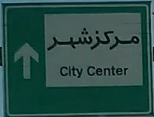
\includegraphics[width=35mm]{NR.png}
}\hspace{-2mm}
\subfigure[چند مستطیلی \lr{(MR)}]{
\label{fig:MR}
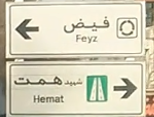
\includegraphics[width=35mm]{MR.png}
}\hspace{-2mm}
\subfigure[پنج ضلعی \lr{(BP/TP)}]{
\label{fig:BP}
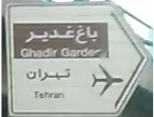
\includegraphics[width=35mm]{BP.png}
}\hspace{-2mm}
\subfigure[پنج ضلعی با پیکان \lr{(AP)}]{
\label{fig:AP}
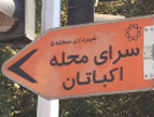
\includegraphics[width=35mm]{AP.png}
}\hspace{-2mm}
\caption{انواع قاب تابلو}
\end{figure}

 \section{اساس روش پیشنهادی و الگوریتم‌های مورد استفاده}
لورم ایپسوم ( به انگلیسی \lr{lorem ipsum} ) متنی بی مفهوم است که تشکیل شده از کلمات معنی دار یا بی معنی کنار هم. کاربر با دیدن متن لورم ایپسوم تصور میکند متنی که در صفحه مشاهده میکند این متن واقعی و مربوط به توضیحات صفحه مورد نظر است واقعی است. حالا سوال اینجاست که این متن « لورم ایپسوم » به چه دردی میخورد و اساسا برای چه منظور و هدفی ساخته شده است؟ پیش از بوجود آمدن لورم ایپسوم ، طراحان وب سایت در پروژه های وب سایت و طراحان کرافیک در پروژه های طراحی کاتولوگ ، بروشور ، پوستر و ... همواره با این مشکل مواجه بودند که صفحات پروژه خود را پیش از آنکه متن اصلی توسط کارفرما ارائه گردد و در صفحه مورد نظر قرار گیرد چگونه پر کنند؟؟ اکثر طراحان با نوشتن یک جمله مانند «این یک متن نمونه است» ویا «توضیحات در این بخش قرار خواهند گرفت» و کپی آن به تعداد زیاد یک یا چند پاراگراف متن میساختند که تمامی متن ها و کلمات ، جملات و پاراگراف ها تکراری بود و از این رو منظره خوبی برای بیننده نداشت و ضمنا به هیچ وجه واقعی به نظر نمیرسید تا بتواند شکل و شمایل تمام شده پروژه را نشان دهد. از این رو متنی ساخته شد که با دو کلمه ( به فارسی : لورم ایپسوم ) آغاز میشد وبا همین نام در بین طراحان وب و گرافیک شناخته و به سرعت محبوب شد. وب سایت های سازنده لورم ایپسوم میتوانند هر تعداد کلمه و پاراگراف که بخواهید به صوورت تکراری یا غیر تکراری برایتان بسازند و تحویلتان بدهند تا از آنها در پروژه هایتان استفاده کنید. ( لورم ایپسوم فارسی) متن های لورم ایپسوم را به زبان فارسی و علاوه بر زبان فارسی به انگلیسی ، عربی ، ترکی استانبولی و ... برایتان میسازد. زبان های دیگر نیز رفته رفته به بانک اطلاعاتی لورم ایسپوم فارسی اضافه خواهند شد.  

\subsection{رنگ}
لورم ایپسوم ( به انگلیسی \lr{lorem ipsum} ) متنی بی مفهوم است که تشکیل شده از کلمات معنی دار یا بی معنی کنار هم. کاربر با دیدن متن لورم ایپسوم تصور میکند متنی که در صفحه مشاهده میکند این متن واقعی و مربوط به توضیحات صفحه مورد نظر است واقعی است. حالا سوال اینجاست که این متن « لورم ایپسوم » به چه دردی میخورد و اساسا برای چه منظور و هدفی ساخته شده است؟ پیش از بوجود آمدن لورم ایپسوم ، طراحان وب سایت در پروژه های وب سایت و طراحان کرافیک در پروژه های طراحی کاتولوگ ، بروشور ، پوستر و ... همواره با این مشکل مواجه بودند که صفحات پروژه خود را پیش از آنکه متن اصلی توسط کارفرما ارائه گردد و در صفحه مورد نظر قرار گیرد چگونه پر کنند؟؟ اکثر طراحان با نوشتن یک جمله مانند «این یک متن نمونه است» ویا «توضیحات در این بخش قرار خواهند گرفت» و کپی آن به تعداد زیاد یک یا چند پاراگراف متن میساختند که تمامی متن ها و کلمات ، جملات و پاراگراف ها تکراری بود و از این رو منظره خوبی برای بیننده نداشت و ضمنا به هیچ وجه واقعی به نظر نمیرسید تا بتواند شکل و شمایل تمام شده پروژه را نشان دهد. از این رو متنی ساخته شد که با دو کلمه ( به فارسی : لورم ایپسوم ) آغاز میشد وبا همین نام در بین طراحان وب و گرافیک شناخته و به سرعت محبوب شد. وب سایت های سازنده لورم ایپسوم میتوانند هر تعداد کلمه و پاراگراف که بخواهید به صوورت تکراری یا غیر تکراری برایتان بسازند و تحویلتان بدهند تا از آنها در پروژه هایتان استفاده کنید. ( لورم ایپسوم فارسی) متن های لورم ایپسوم را به زبان فارسی و علاوه بر زبان فارسی به انگلیسی ، عربی ، ترکی استانبولی و ... برایتان میسازد. زبان های دیگر نیز رفته رفته به بانک اطلاعاتی لورم ایسپوم فارسی اضافه خواهند شد.  


\begin{figure}[!htb]
\centering     %%% not \center
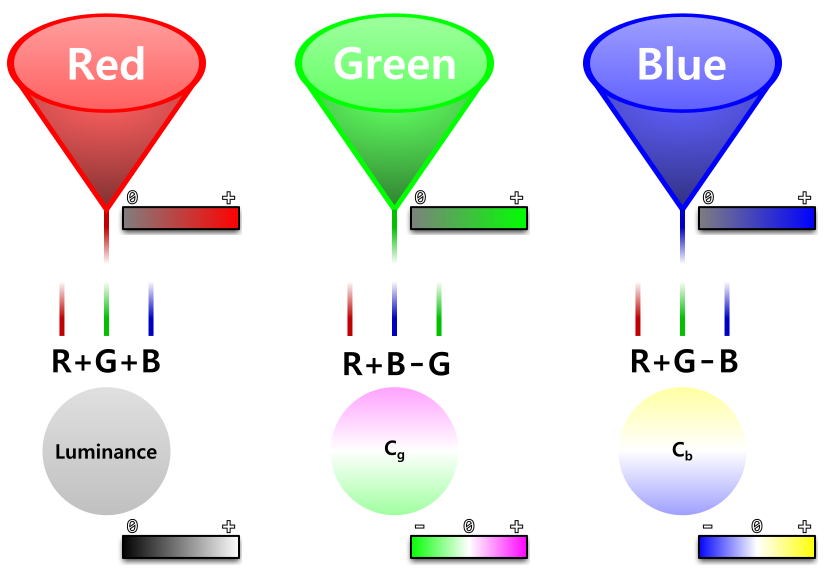
\includegraphics[height=70mm]{oppcolor.png}
\caption[رنگ‌های مخالف]{
پردازش رنگ‌های مخالف در بینایی رنگ \cite{ wiki:hsl}
}
\label{fig:oppcolor}
\end{figure}


\begin{figure}[htb]
\centering     %%% not \center
\subfigure[فیلتر رنگ سفید]{
\label{fig:w}
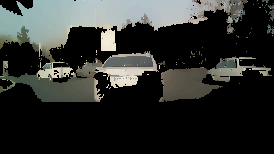
\includegraphics[height=35mm]{w2.png}
}\hspace{-2mm}
\subfigure[فیلتر رنگ سبز]{
\label{fig:g}

\includegraphics[height=35mm]{g2.png}
}
\caption{نمونه فیلترهای رنگ}
\label{fig:color}
\end{figure}


\subsection{روش فلان}

لورم ایپسوم ( به انگلیسی \lr{lorem ipsum} ) متنی بی مفهوم است که تشکیل شده از کلمات معنی دار یا بی معنی کنار هم. کاربر با دیدن متن لورم ایپسوم تصور میکند متنی که در صفحه مشاهده میکند این متن واقعی و مربوط به توضیحات صفحه مورد نظر است واقعی است. حالا سوال اینجاست که این متن « لورم ایپسوم » به چه دردی میخورد و اساسا برای چه منظور و هدفی ساخته شده است؟ پیش از بوجود آمدن لورم ایپسوم ، طراحان وب سایت در پروژه های وب سایت و طراحان کرافیک در پروژه های طراحی کاتولوگ ، بروشور ، پوستر و ... همواره با این مشکل مواجه بودند که صفحات پروژه خود را پیش از آنکه متن اصلی توسط کارفرما ارائه گردد و در صفحه مورد نظر قرار گیرد چگونه پر کنند؟؟ اکثر طراحان با نوشتن یک جمله مانند «این یک متن نمونه است» ویا «توضیحات در این بخش قرار خواهند گرفت» و کپی آن به تعداد زیاد یک یا چند پاراگراف متن میساختند که تمامی متن ها و کلمات ، جملات و پاراگراف ها تکراری بود و از این رو منظره خوبی برای بیننده نداشت و ضمنا به هیچ وجه واقعی به نظر نمیرسید تا بتواند شکل و شمایل تمام شده پروژه را نشان دهد. از این رو متنی ساخته شد که با دو کلمه ( به فارسی : لورم ایپسوم ) آغاز میشد وبا همین نام در بین طراحان وب و گرافیک شناخته و به سرعت محبوب شد. وب سایت های سازنده لورم ایپسوم میتوانند هر تعداد کلمه و پاراگراف که بخواهید به صوورت تکراری یا غیر تکراری برایتان بسازند و تحویلتان بدهند تا از آنها در پروژه هایتان استفاده کنید. ( لورم ایپسوم فارسی) متن های لورم ایپسوم را به زبان فارسی و علاوه بر زبان فارسی به انگلیسی ، عربی ، ترکی استانبولی و ... برایتان میسازد. زبان های دیگر نیز رفته رفته به بانک اطلاعاتی لورم ایسپوم فارسی اضافه خواهند شد.  

\begin{equation}
\begin{aligned}
\mathcal{A}(f) & = \mathfrak{R} \Big( \mathfrak{F} \big[ \mathcal{I}(x) \big] \Big), \\
\mathcal{P}(f) & = \mathfrak{I} \Big( \mathfrak{F} \big[ \mathcal{I}(x) \big] \Big), \\
\mathcal{L}(f) & = \log \Big( \mathcal{A}(f) \Big) , \\
\mathcal{R}(f) & =  \mathcal{L}(f) - h_n(f) \ast  \mathcal{L}(f) ,\\
\mathcal{S}(x) & = g(x) \ast \mathfrak{F}^{-1} \Big[ \exp \big(  \mathcal{R}(f) + \mathcal{P}(f) \big) \Big]^{2} \quad . 
\end{aligned}
\end{equation}
تبدیل فوریه با 
$\mathfrak{F}$
نشان داده شده‌است که بخش حقیقی آن 
$\mathfrak{R}$
، بخش مختلط آن (فاز) 
$\mathfrak{I}$
و
$\mathfrak{F}^{-1}$
تبدیل معکوس فوریه است. همچنین 
 $\mathcal{R}(f)$
  باقی‌مانده‌ی طیفی، 
 $\mathcal{S}(x)$
  نقشه‌ 
 $g(x)$
  فیلتر گاوسی و $h_n$ همانند \eqref{eq:hn} با
   $n=3$
    است. 
\begin{equation}
h_n = {{1} \over {n^2} } 
{
\renewcommand\arraystretch{0.5}
 \begin{pmatrix}
    1 & 1 & \cdots & 1  \\
	1 & 1 & \cdots & 1 \\
	 \vdots & \vdots& \ddots & \vdots  \\
	     1 & 1 & \cdots & 1  \\
  \end{pmatrix}
}
\label{eq:hn}
\end{equation}
	
لورم ایپسوم ( به انگلیسی \lr{lorem ipsum} ) متنی بی مفهوم است که تشکیل شده از کلمات معنی دار یا بی معنی کنار هم. کاربر با دیدن متن لورم ایپسوم تصور میکند متنی که در صفحه مشاهده میکند این متن واقعی و مربوط به توضیحات صفحه مورد نظر است واقعی است. حالا سوال اینجاست که این متن « لورم ایپسوم » به چه دردی میخورد و اساسا برای چه منظور و هدفی ساخته شده است؟ پیش از بوجود آمدن لورم ایپسوم ، طراحان وب سایت در پروژه های وب سایت و طراحان کرافیک در پروژه های طراحی کاتولوگ ، بروشور ، پوستر و ... همواره با این مشکل مواجه بودند که صفحات پروژه خود را پیش از آنکه متن اصلی توسط کارفرما ارائه گردد و در صفحه مورد نظر قرار گیرد چگونه پر کنند؟؟ اکثر طراحان با نوشتن یک جمله مانند «این یک متن نمونه است» ویا «توضیحات در این بخش قرار خواهند گرفت» و کپی آن به تعداد زیاد یک یا چند پاراگراف متن میساختند که تمامی متن ها و کلمات ، جملات و پاراگراف ها تکراری بود و از این رو منظره خوبی برای بیننده نداشت و ضمنا به هیچ وجه واقعی به نظر نمیرسید تا بتواند شکل و شمایل تمام شده پروژه را نشان دهد. از این رو متنی ساخته شد که با دو کلمه ( به فارسی : لورم ایپسوم ) آغاز میشد وبا همین نام در بین طراحان وب و گرافیک شناخته و به سرعت محبوب شد. وب سایت های سازنده لورم ایپسوم میتوانند هر تعداد کلمه و پاراگراف که بخواهید به صوورت تکراری یا غیر تکراری برایتان بسازند و تحویلتان بدهند تا از آنها در پروژه هایتان استفاده کنید. ( لورم ایپسوم فارسی) متن های لورم ایپسوم را به زبان فارسی و علاوه بر زبان فارسی به انگلیسی ، عربی ، ترکی استانبولی و ... برایتان میسازد. زبان های دیگر نیز رفته رفته به بانک اطلاعاتی لورم ایسپوم فارسی اضافه خواهند شد.  

\begin{figure}[p]
\centering     %%% not \center
\subfigure[تصویر اصلی]{
\label{fig:s1}
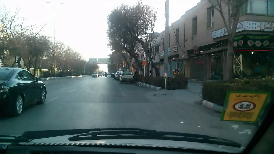
\includegraphics[height=35mm]{s1.png}
}\hspace{-2mm}
\subfigure[نقشه]{
\label{fig:s1o}
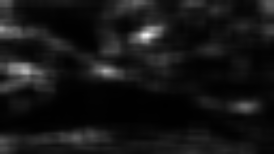
\includegraphics[height=35mm]{s1o.png}
}
\subfigure[تصویر اصلی]{
\label{fig:s2}
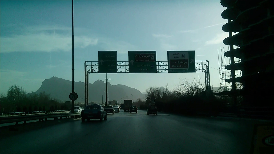
\includegraphics[height=35mm]{s2.png}
}\hspace{-2mm}
\subfigure[نقشه]{
\label{fig:s2o}
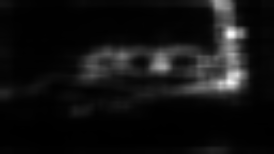
\includegraphics[height=35mm]{s2o.png}
}
\subfigure[تصویر اصلی]{
\label{fig:s3}
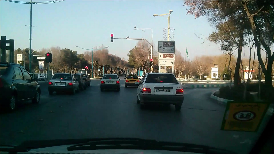
\includegraphics[height=35mm]{s3.png}
}\hspace{-2mm}
\subfigure[نقشه]{
\label{fig:s3o}
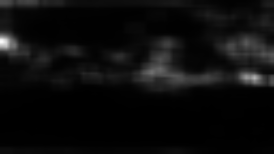
\includegraphics[height=35mm]{s3o.png}
}
\caption[نمونه نقشه‌ها]
{نقشه‌ها در محیط شهری}
\end{figure}
لورم ایپسوم ( به انگلیسی \lr{lorem ipsum} ) متنی بی مفهوم است که تشکیل شده از کلمات معنی دار یا بی معنی کنار هم. کاربر با دیدن متن لورم ایپسوم تصور میکند متنی که در صفحه مشاهده میکند این متن واقعی و مربوط به توضیحات صفحه مورد نظر است واقعی است. حالا سوال اینجاست که این متن « لورم ایپسوم » به چه دردی میخورد و اساسا برای چه منظور و هدفی ساخته شده است؟ پیش از بوجود آمدن لورم ایپسوم ، طراحان وب سایت در پروژه های وب سایت و طراحان کرافیک در پروژه های طراحی کاتولوگ ، بروشور ، پوستر و ... همواره با این مشکل مواجه بودند که صفحات پروژه خود را پیش از آنکه متن اصلی توسط کارفرما ارائه گردد و در صفحه مورد نظر قرار گیرد چگونه پر کنند؟؟ اکثر طراحان با نوشتن یک جمله مانند «این یک متن نمونه است» ویا «توضیحات در این بخش قرار خواهند گرفت» و کپی آن به تعداد زیاد یک یا چند پاراگراف متن میساختند که تمامی متن ها و کلمات ، جملات و پاراگراف ها تکراری بود و از این رو منظره خوبی برای بیننده نداشت و ضمنا به هیچ وجه واقعی به نظر نمیرسید تا بتواند شکل و شمایل تمام شده پروژه را نشان دهد. از این رو متنی ساخته شد که با دو کلمه ( به فارسی : لورم ایپسوم ) آغاز میشد وبا همین نام در بین طراحان وب و گرافیک شناخته و به سرعت محبوب شد. وب سایت های سازنده لورم ایپسوم میتوانند هر تعداد کلمه و پاراگراف که بخواهید به صوورت تکراری یا غیر تکراری برایتان بسازند و تحویلتان بدهند تا از آنها در پروژه هایتان استفاده کنید. ( لورم ایپسوم فارسی) متن های لورم ایپسوم را به زبان فارسی و علاوه بر زبان فارسی به انگلیسی ، عربی ، ترکی استانبولی و ... برایتان میسازد. زبان های دیگر نیز رفته رفته به بانک اطلاعاتی لورم ایسپوم فارسی اضافه خواهند شد.  


سیگنال یک بعدی
 $I : \Omega \rightarrow \mathbb{R}, \Omega = [0 , \infty ) \subset \mathbb{R}$ 
 یک خم $C$ در فضای $\mathbb{R}^2$ می‌سازد. تبدیل ارایه‌شده خم $C$ را از فضایisometric $\mathbb{R}^2$ به فضای $\mathbb{R}$ تبدیل می‌کند به گونه‌ای که فاصله‌ی نقاط اصلی روی خم $C$ با در نظر گرفتن معیاری، حفظ می‌شود. این معیار نرم $l_1$ در نظر گرفته شده‌است، به این معنی که فاصله‌ی نقاط همسایه در تبدیل جدید $(\mathbb{R})$ باید برابر با فاصله‌ی $l_1$ آن‌ها در دامنه‌ی اصلی $(\mathbb{R}^2)$ باشد. تبدیل 
 $ct(x) = t(\hat{x}) = t(x , I(x))$
 را فرض می‌کنیم. لورم ایپسوم ( به انگلیسی \lr{lorem ipsum} ) متنی بی مفهوم است که تشکیل شده از کلمات معنی دار یا بی معنی کنار هم. کاربر با دیدن متن لورم ایپسوم تصور میکند متنی که در صفحه مشاهده میکند این متن واقعی و مربوط به توضیحات صفحه مورد نظر است واقعی است. حالا سوال اینجاست که این متن « لورم ایپسوم » به چه دردی میخورد و اساسا برای چه منظور و هدفی ساخته شده است؟ پیش از بوجود آمدن لورم ایپسوم ، طراحان وب سایت در پروژه های وب سایت و طراحان کرافیک در پروژه های طراحی کاتولوگ ، بروشور ، پوستر و ... همواره با این مشکل مواجه بودند که صفحات پروژه خود را پیش از آنکه متن اصلی توسط کارفرما ارائه گردد و در صفحه مورد نظر قرار گیرد چگونه پر کنند؟؟ اکثر طراحان با نوشتن یک جمله مانند «این یک متن نمونه است» ویا «توضیحات در این بخش قرار خواهند گرفت» و کپی آن به تعداد زیاد یک یا چند پاراگراف متن میساختند که تمامی متن ها و کلمات ، جملات و پاراگراف ها تکراری بود و از این رو منظره خوبی برای بیننده نداشت و ضمنا به هیچ وجه واقعی به نظر نمیرسید تا بتواند شکل و شمایل تمام شده پروژه را نشان دهد. از این رو متنی ساخته شد که با دو کلمه ( به فارسی : لورم ایپسوم ) آغاز میشد وبا همین نام در بین طراحان وب و گرافیک شناخته و به سرعت محبوب شد. وب سایت های سازنده لورم ایپسوم میتوانند هر تعداد کلمه و پاراگراف که بخواهید به صوورت تکراری یا غیر تکراری برایتان بسازند و تحویلتان بدهند تا از آنها در پروژه هایتان استفاده کنید. ( لورم ایپسوم فارسی) متن های لورم ایپسوم را به زبان فارسی و علاوه بر زبان فارسی به انگلیسی ، عربی ، ترکی استانبولی و ... برایتان میسازد. زبان های دیگر نیز رفته رفته به بانک اطلاعاتی لورم ایسپوم فارسی اضافه خواهند شد.  

لورم ایپسوم ( به انگلیسی \lr{lorem ipsum} ) متنی بی مفهوم است که تشکیل شده از کلمات معنی دار یا بی معنی کنار هم. کاربر با دیدن متن لورم ایپسوم تصور میکند متنی که در صفحه مشاهده میکند این متن واقعی و مربوط به توضیحات صفحه مورد نظر است واقعی است. حالا سوال اینجاست که این متن « لورم ایپسوم » به چه دردی میخورد و اساسا برای چه منظور و هدفی ساخته شده است؟ پیش از بوجود آمدن لورم ایپسوم ، طراحان وب سایت در پروژه های وب سایت و طراحان کرافیک در پروژه های طراحی کاتولوگ ، بروشور ، پوستر و ... همواره با این مشکل مواجه بودند که صفحات پروژه خود را پیش از آنکه متن اصلی توسط کارفرما ارائه گردد و در صفحه مورد نظر قرار گیرد چگونه پر کنند؟؟ اکثر طراحان با نوشتن یک جمله مانند «این یک متن نمونه است» ویا «توضیحات در این بخش قرار خواهند گرفت» و کپی آن به تعداد زیاد یک یا چند پاراگراف متن میساختند که تمامی متن ها و کلمات ، جملات و پاراگراف ها تکراری بود و از این رو منظره خوبی برای بیننده نداشت و ضمنا به هیچ وجه واقعی به نظر نمیرسید تا بتواند شکل و شمایل تمام شده پروژه را نشان دهد. از این رو متنی ساخته شد که با دو کلمه ( به فارسی : لورم ایپسوم ) آغاز میشد وبا همین نام در بین طراحان وب و گرافیک شناخته و به سرعت محبوب شد. وب سایت های سازنده لورم ایپسوم میتوانند هر تعداد کلمه و پاراگراف که بخواهید به صوورت تکراری یا غیر تکراری برایتان بسازند و تحویلتان بدهند تا از آنها در پروژه هایتان استفاده کنید. ( لورم ایپسوم فارسی) متن های لورم ایپسوم را به زبان فارسی و علاوه بر زبان فارسی به انگلیسی ، عربی ، ترکی استانبولی و ... برایتان میسازد. زبان های دیگر نیز رفته رفته به بانک اطلاعاتی لورم ایسپوم فارسی اضافه خواهند شد.  


 \begin{equation}
 D(C_1, C_2) = 
 \begin{cases}
    \textit{\lr{true}} & \text{\lr{if} } \ Dif(C_1, C_2) > MInt(C_1, C_2)\\
    false & \text{otherwise}
\end{cases}
 \end{equation}
 
 که در آن کمینه تفاوت داخلی $MInt$ به این صورت تعریف می‌شود‌: 
 \begin{equation}
 MInt(C_1, C_2) = min (Int(C_1) + \tau (C_1), Int(C_2) + \tau (C_2))
 \end{equation}
لورم ایپسوم ( به انگلیسی \lr{lorem ipsum} ) متنی بی مفهوم است که تشکیل شده از کلمات معنی دار یا بی معنی کنار هم. کاربر با دیدن متن لورم ایپسوم تصور میکند متنی که در صفحه مشاهده میکند این متن واقعی و مربوط به توضیحات صفحه مورد نظر است واقعی است. حالا سوال اینجاست که این متن « لورم ایپسوم » به چه دردی میخورد و اساسا برای چه منظور و هدفی ساخته شده است؟ پیش از بوجود آمدن لورم ایپسوم ، طراحان وب سایت در پروژه های وب سایت و طراحان کرافیک در پروژه های طراحی کاتولوگ ، بروشور ، پوستر و ... همواره با این مشکل مواجه بودند که صفحات پروژه خود را پیش از آنکه متن اصلی توسط کارفرما ارائه گردد و در صفحه مورد نظر قرار گیرد چگونه پر کنند؟؟ اکثر طراحان با نوشتن یک جمله مانند «این یک متن نمونه است» ویا «توضیحات در این بخش قرار خواهند گرفت» و کپی آن به تعداد زیاد یک یا چند پاراگراف متن میساختند که تمامی متن ها و کلمات ، جملات و پاراگراف ها تکراری بود و از این رو منظره خوبی برای بیننده نداشت و ضمنا به هیچ وجه واقعی به نظر نمیرسید تا بتواند شکل و شمایل تمام شده پروژه را نشان دهد. از این رو متنی ساخته شد که با دو کلمه ( به فارسی : لورم ایپسوم ) آغاز میشد وبا همین نام در بین طراحان وب و گرافیک شناخته و به سرعت محبوب شد. وب سایت های سازنده لورم ایپسوم میتوانند هر تعداد کلمه و پاراگراف که بخواهید به صوورت تکراری یا غیر تکراری برایتان بسازند و تحویلتان بدهند تا از آنها در پروژه هایتان استفاده کنید. ( لورم ایپسوم فارسی) متن های لورم ایپسوم را به زبان فارسی و علاوه بر زبان فارسی به انگلیسی ، عربی ، ترکی استانبولی و ... برایتان میسازد. زبان های دیگر نیز رفته رفته به بانک اطلاعاتی لورم ایسپوم فارسی اضافه خواهند شد.  

 
 \begin{equation}
 \begin{aligned}
 C_{ab}^* & = \sqrt{a^{*2} + b^{*2}} ,\quad h_{ab} = \arctan \frac{b^{*}}{a^{*}}\\
 \Delta E_{94}^* & = \sqrt{ \left(\frac{\Delta L^*}{k_L S_L}\right)^2 + \left(\frac{\Delta C^*_{ab}}{k_C S_C}\right)^2 + \left(\frac{\Delta H^*_{ab}}{k_H S_H}\right)^2 }, \quad where:\\
 \Delta L^* &= L^*_1 - L^*_2 ,\quad C^*_1 = \sqrt{ {a^*_1}^2 + {b^*_1}^2 } ,\\
 C^*_2 &= \sqrt{ {a^*_2}^2 + {b^*_2}^2 } ,\quad \Delta C^*_{ab} = C^*_1 - C^*_2 \\
 \Delta H^*_{ab} & = \sqrt{ {\Delta E^*_{ab}}^2 - {\Delta L^*}^2 - {\Delta C^*_{ab}}^2 } = \sqrt{ {\Delta a^*}^2 + {\Delta b^*}^2 - {\Delta C^*_{ab}}^2 }\\
 \Delta a^* & = a^*_1 - a^*_2 ,\quad \Delta b^* = b^*_1 - b^*_2, \quad S_L = 1 , \quad S_C = 1+K_1 C^*_1 ,\\
  S_H & = 1+K_2 C^*_1, \quad k_L = 1 , \quad K_1 = 0.045, \quad K_2 = 0.015
  \end{aligned}
 \end{equation}
لورم ایپسوم ( به انگلیسی \lr{lorem ipsum} ) متنی بی مفهوم است که تشکیل شده از کلمات معنی دار یا بی معنی کنار هم. کاربر با دیدن متن لورم ایپسوم تصور میکند متنی که در صفحه مشاهده میکند این متن واقعی و مربوط به توضیحات صفحه مورد نظر است واقعی است. حالا سوال اینجاست که این متن « لورم ایپسوم » به چه دردی میخورد و اساسا برای چه منظور و هدفی ساخته شده است؟ پیش از بوجود آمدن لورم ایپسوم ، طراحان وب سایت در پروژه های وب سایت و طراحان کرافیک در پروژه های طراحی کاتولوگ ، بروشور ، پوستر و ... همواره با این مشکل مواجه بودند که صفحات پروژه خود را پیش از آنکه متن اصلی توسط کارفرما ارائه گردد و در صفحه مورد نظر قرار گیرد چگونه پر کنند؟؟ اکثر طراحان با نوشتن یک جمله مانند «این یک متن نمونه است» ویا «توضیحات در این بخش قرار خواهند گرفت» و کپی آن به تعداد زیاد یک یا چند پاراگراف متن میساختند که تمامی متن ها و کلمات ، جملات و پاراگراف ها تکراری بود و از این رو منظره خوبی برای بیننده نداشت و ضمنا به هیچ وجه واقعی به نظر نمیرسید تا بتواند شکل و شمایل تمام شده پروژه را نشان دهد. از این رو متنی ساخته شد که با دو کلمه ( به فارسی : لورم ایپسوم ) آغاز میشد وبا همین نام در بین طراحان وب و گرافیک شناخته و به سرعت محبوب شد. وب سایت های سازنده لورم ایپسوم میتوانند هر تعداد کلمه و پاراگراف که بخواهید به صوورت تکراری یا غیر تکراری برایتان بسازند و تحویلتان بدهند تا از آنها در پروژه هایتان استفاده کنید. ( لورم ایپسوم فارسی) متن های لورم ایپسوم را به زبان فارسی و علاوه بر زبان فارسی به انگلیسی ، عربی ، ترکی استانبولی و ... برایتان میسازد. زبان های دیگر نیز رفته رفته به بانک اطلاعاتی لورم ایسپوم فارسی اضافه خواهند شد.  
 
%------------------------ End chapter 3 -------------


\cchapter{ارزیابی}
\label{chap:result}
\pagebreak

\section{مقدمه}

در این بخش پس از معرفی مجموعه‌دادگان تهیه‌شده \cite{khazaee2016aut}، بررسی مزایا و معایب روش پیشنهادی صورت گرفته‌است. از آن‌جا که پژوهش‌های انجام شده‌ در این زمینه هر کدام روش متفاوتی برای تعریف صورت مساله و در نتیجه ارزیابی عملکرد متفاوتی ارایه نموده‌اند، تلاش بر آن بوده‌است که جنبه‌های مشترک با هر یک از این پژوهش‌ها تحت بررسی قرار گیرد. لازم به یاد آوری است که تا کنون مجموعه‌دادگان مشخص و برچسب‌گذاری شده برای این مساله وجود نداشته است و این خود به پراکندگی و ابهام روش‌های ارزیابی منجر شده‌است. از طرفی، این مساله در محیط شلوغ شهری با پوشش رنگ سفید برای اولین بار تعریف شده است و ارزیابی مستقیم با روش‌های موجود امکان پذیر نیست. همچنین، تلاش اصلی ما در این پژوهش برای بی‌درنگ انجام دادن کار بوده است تا زمان کافی برای اجرای دیگر الگوریتم‌های هم‌یاری راننده از جمله الگوریتم‌های شناسایی حروف وجود داشته باشد. با توجه به این نکته، چالش اصلی در پژوهش ما انتخاب ترجیح مناسب بین کارایی و صحت بوده است. از این رو لازم است قبل از پرداختن به ارزیابی کمی، تفاوت‌های کیفی با پژوهش‌های موجود و تفاوت‌ها در نحوه‌ی ارزیابی بیان شود. در ادامه به بحث بر روی معیارهای ارزیابی پرداخته شده‌است و در بخش‌های آتی ارزیابی‌های کمی ارایه شده‌اند. 


\section{مجموعه دادگان}

این مجموعه از ۱۳۴۳۲۸ فریم تصویر تشکیل شده‌است که توسط یک دوربین نصب شده در خودروی در حال حرکت در محیط شهری با کیفیت $1920 \times 1080$ تهیه شده‌است و سپس دادگان برای اولین‌بار در حجم بالا توسط انسان برچسب‌گذاری شده است تا داده‌ی زمینه‌ی استاندارد موجود باشد. همچنین تحلیل آماری و دسته‌بندی‌های لازم انجام شده‌است که به جزییات آن خواهیم پرداخت. این ویدیوها شامل بخش‌هایی که تابلوی راهنما در آن وجود ندارد نیز می‌شوند، اما به دلیل چالشی بودن، بعضی از این ویدیوها که گاهی طولانی هم هستند حذف نشده‌اند تا مجموعه دادگان به مساله در دنیای واقعی نزدیک‌تر باشد. از جمله‌ی این چالش‌ها می‌توان به وجود برخی نواحی سفید، بنرهای تبلیغاتی، و دیگر تابلوهای موجود در محیط شهری اشاره کرد. برخی نمونه‌های این چالش‌ها در تصویر \ref{fig:chall1} آورده‌ شده‌اند. 
\begin{figure}[ht]
\centering
    	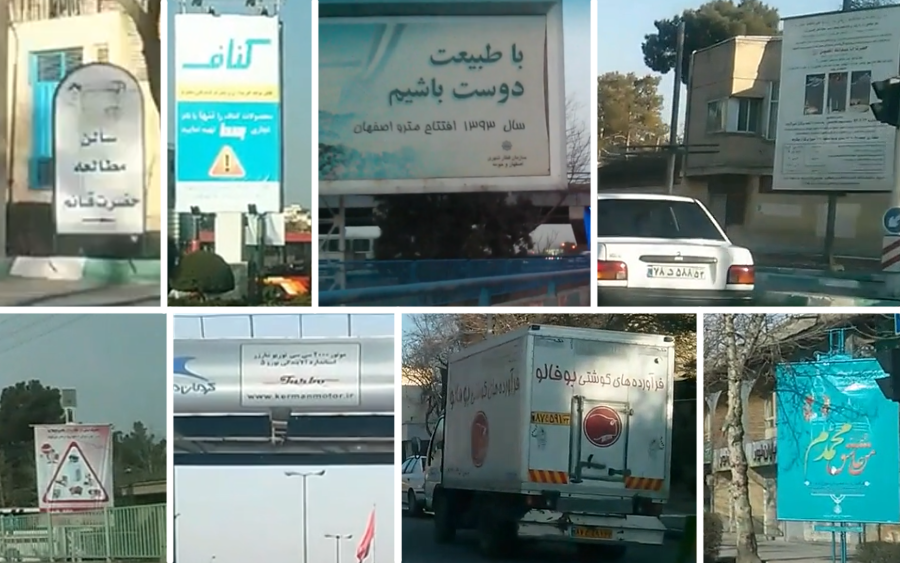
\includegraphics[width=13cm]{Figures/chall1.png}
\caption{برخی چالش‌های ساختاری در محیط شهری}
\label{fig:chall1}
\end{figure}
با این وجود، دنباله‌های کوتاه‌تری از ویدیوها شامل حداقل یک تابلوی راهنما در هر دنباله نیز تهیه شده‌است که در مجموع شامل ۲۶۹۸۸ فریم می‌شود. این دنباله‌ها در فاصله‌ای از تابلو شروع می‌شوند که انتظار می‌رود سیستم هوشمند در بهترین حالت از آن فاصله تشخیص را آغاز کند. پژوهشگران می‌توانند از این مجموعه‌ی کوتاه‌تر برای آموزش و آزمون روش خود استفاده کنند. 

برای مقایسه، به شکل‌های
 \ref{fig:compdb1}
  و \ref{fig:compdb2}
  مراجعه کنید. در این تصاویر مجموعه‌دادگان تهیه شده با تنها مجموعه دادگان موجود (میرمهدی \cite{Greenhalgh2015}) مقایسه شده‌است. از نظر تعداد، مجموعه دادگان تهیه شده به میزان قابل توجهی بزرگ‌تر از مجموعه‌های استفاده‌شده تا کنون است. برای نمونه، مجموعه‌ی معرفی شده توسط میرمهدی به طور تقریبی شامل ۴۸ هزار فریم است که دنباله‌های طولانی از آن بدون تابلوی راهنما هستند. 
\begin{figure}[p]
\centering
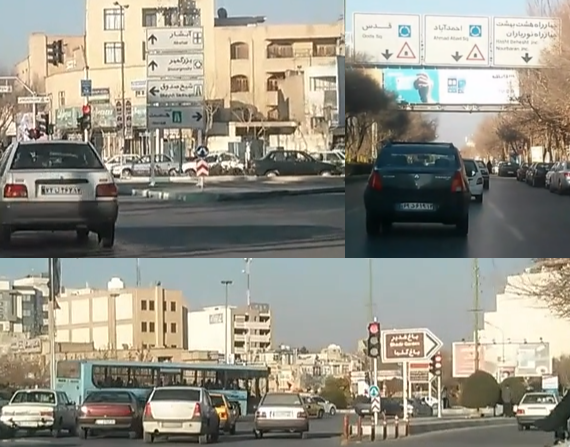
\includegraphics[height=9cm]{Figures/real.png}
\caption{نمونه دادگان تهیه شده}
\label{fig:compdb1}
\vspace{3mm}
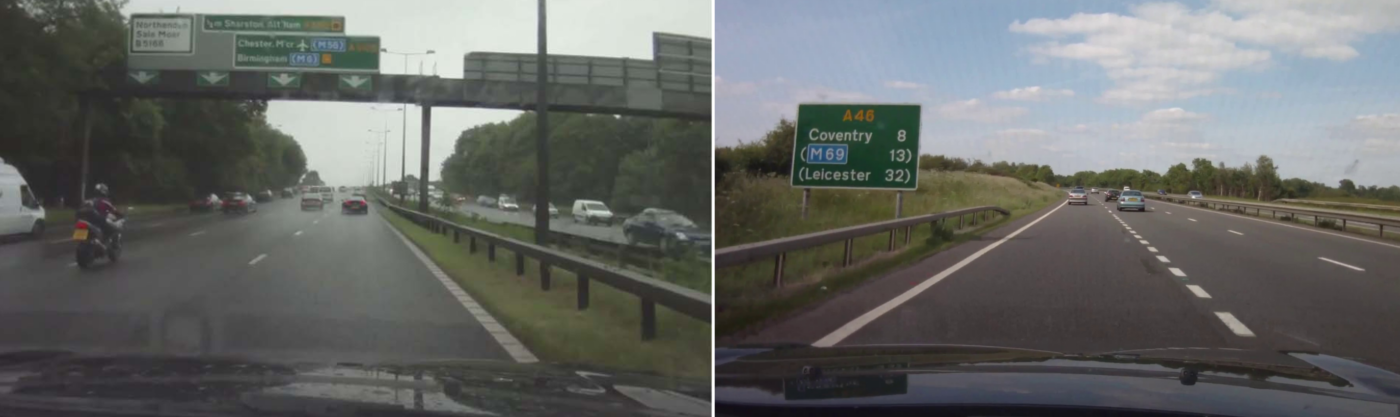
\includegraphics[height=3.5cm]{Figures/mirmdb1.png}
\caption{نمونه دادگان موجود}
\label{fig:compdb2}
\end{figure}

\subsection{ویژگی‌های مجموعه دادگان}
\label{subsec:dbattr}

لورم ایپسوم ( به انگلیسی \lr{lorem ipsum} ) متنی بی مفهوم است که تشکیل شده از کلمات معنی دار یا بی معنی کنار هم. کاربر با دیدن متن لورم ایپسوم تصور میکند متنی که در صفحه مشاهده میکند این متن واقعی و مربوط به توضیحات صفحه مورد نظر است واقعی است. حالا سوال اینجاست که این متن « لورم ایپسوم » به چه دردی میخورد و اساسا برای چه منظور و هدفی ساخته شده است؟ پیش از بوجود آمدن لورم ایپسوم ، طراحان وب سایت در پروژه های وب سایت و طراحان کرافیک در پروژه های طراحی کاتولوگ ، بروشور ، پوستر و ... همواره با این مشکل مواجه بودند که صفحات پروژه خود را پیش از آنکه متن اصلی توسط کارفرما ارائه گردد و در صفحه مورد نظر قرار گیرد چگونه پر کنند؟؟ اکثر طراحان با نوشتن یک جمله مانند «این یک متن نمونه است» ویا «توضیحات در این بخش قرار خواهند گرفت» و کپی آن به تعداد زیاد یک یا چند پاراگراف متن میساختند که تمامی متن ها و کلمات ، جملات و پاراگراف ها تکراری بود و از این رو منظره خوبی برای بیننده نداشت و ضمنا به هیچ وجه واقعی به نظر نمیرسید تا بتواند شکل و شمایل تمام شده پروژه را نشان دهد. از این رو متنی ساخته شد که با دو کلمه ( به فارسی : لورم ایپسوم ) آغاز میشد وبا همین نام در بین طراحان وب و گرافیک شناخته و به سرعت محبوب شد. وب سایت های سازنده لورم ایپسوم میتوانند هر تعداد کلمه و پاراگراف که بخواهید به صوورت تکراری یا غیر تکراری برایتان بسازند و تحویلتان بدهند تا از آنها در پروژه هایتان استفاده کنید. ( لورم ایپسوم فارسی) متن های لورم ایپسوم را به زبان فارسی و علاوه بر زبان فارسی به انگلیسی ، عربی ، ترکی استانبولی و ... برایتان میسازد. زبان های دیگر نیز رفته رفته به بانک اطلاعاتی لورم ایسپوم فارسی اضافه خواهند شد.  

\subsection{گزارش آماری}

در این بخش یک تحلیل آماری بر روی مجموعه دادگان ارایه شده است تا محققان ب­توانند شرایط و دسته‌ی مناسب برای مطالعه‌­ی خود را انتخاب کنند. تعداد کل فریم‌ها در نمونه‌ی کوچک و اصلاح‌شده‌ی مجموعه‌دادگان برابر با 12996 است که 5040 فریم آن به صورت دستی اصلاح شده‌است و شامل 10855 بار اصلاح دستی است. 

\section{آزمایش اول: تاثیر فلان کار}
لورم ایپسوم ( به انگلیسی \lr{lorem ipsum} ) متنی بی مفهوم است که تشکیل شده از کلمات معنی دار یا بی معنی کنار هم. کاربر با دیدن متن لورم ایپسوم تصور میکند متنی که در صفحه مشاهده میکند این متن واقعی و مربوط به توضیحات صفحه مورد نظر است واقعی است. حالا سوال اینجاست که این متن « لورم ایپسوم » به چه دردی میخورد و اساسا برای چه منظور و هدفی ساخته شده است؟ پیش از بوجود آمدن لورم ایپسوم ، طراحان وب سایت در پروژه های وب سایت و طراحان کرافیک در پروژه های طراحی کاتولوگ ، بروشور ، پوستر و ... همواره با این مشکل مواجه بودند که صفحات پروژه خود را پیش از آنکه متن اصلی توسط کارفرما ارائه گردد و در صفحه مورد نظر قرار گیرد چگونه پر کنند؟؟ اکثر طراحان با نوشتن یک جمله مانند «این یک متن نمونه است» ویا «توضیحات در این بخش قرار خواهند گرفت» و کپی آن به تعداد زیاد یک یا چند پاراگراف متن میساختند که تمامی متن ها و کلمات ، جملات و پاراگراف ها تکراری بود و از این رو منظره خوبی برای بیننده نداشت و ضمنا به هیچ وجه واقعی به نظر نمیرسید تا بتواند شکل و شمایل تمام شده پروژه را نشان دهد. از این رو متنی ساخته شد که با دو کلمه ( به فارسی : لورم ایپسوم ) آغاز میشد وبا همین نام در بین طراحان وب و گرافیک شناخته و به سرعت محبوب شد. وب سایت های سازنده لورم ایپسوم میتوانند هر تعداد کلمه و پاراگراف که بخواهید به صوورت تکراری یا غیر تکراری برایتان بسازند و تحویلتان بدهند تا از آنها در پروژه هایتان استفاده کنید. ( لورم ایپسوم فارسی) متن های لورم ایپسوم را به زبان فارسی و علاوه بر زبان فارسی به انگلیسی ، عربی ، ترکی استانبولی و ... برایتان میسازد. زبان های دیگر نیز رفته رفته به بانک اطلاعاتی لورم ایسپوم فارسی اضافه خواهند شد.  

\section{آزمایش سوم: تاثیر تبدیل}

لورم ایپسوم ( به انگلیسی \lr{lorem ipsum} ) متنی بی مفهوم است که تشکیل شده از کلمات معنی دار یا بی معنی کنار هم. کاربر با دیدن متن لورم ایپسوم تصور میکند متنی که در صفحه مشاهده میکند این متن واقعی و مربوط به توضیحات صفحه مورد نظر است واقعی است. حالا سوال اینجاست که این متن « لورم ایپسوم » به چه دردی میخورد و اساسا برای چه منظور و هدفی ساخته شده است؟ پیش از بوجود آمدن لورم ایپسوم ، طراحان وب سایت در پروژه های وب سایت و طراحان کرافیک در پروژه های طراحی کاتولوگ ، بروشور ، پوستر و ... همواره با این مشکل مواجه بودند که صفحات پروژه خود را پیش از آنکه متن اصلی توسط کارفرما ارائه گردد و در صفحه مورد نظر قرار گیرد چگونه پر کنند؟؟ اکثر طراحان با نوشتن یک جمله مانند «این یک متن نمونه است» ویا «توضیحات در این بخش قرار خواهند گرفت» و کپی آن به تعداد زیاد یک یا چند پاراگراف متن میساختند که تمامی متن ها و کلمات ، جملات و پاراگراف ها تکراری بود و از این رو منظره خوبی برای بیننده نداشت و ضمنا به هیچ وجه واقعی به نظر نمیرسید تا بتواند شکل و شمایل تمام شده پروژه را نشان دهد. از این رو متنی ساخته شد که با دو کلمه ( به فارسی : لورم ایپسوم ) آغاز میشد وبا همین نام در بین طراحان وب و گرافیک شناخته و به سرعت محبوب شد. وب سایت های سازنده لورم ایپسوم میتوانند هر تعداد کلمه و پاراگراف که بخواهید به صوورت تکراری یا غیر تکراری برایتان بسازند و تحویلتان بدهند تا از آنها در پروژه هایتان استفاده کنید. ( لورم ایپسوم فارسی) متن های لورم ایپسوم را به زبان فارسی و علاوه بر زبان فارسی به انگلیسی ، عربی ، ترکی استانبولی و ... برایتان میسازد. زبان های دیگر نیز رفته رفته به بانک اطلاعاتی لورم ایسپوم فارسی اضافه خواهند شد.  

\begin{table}[h]
\begin{center}
\def\arraystretch{1.5}
\begin{tabularx}{\textwidth}{|X|c|c|c|c|}
\hline
 &
 $\bar{s}_{p}$ & $\sigma_p$ & $\bar{s}_{n}$ & $\sigma_p$ \\
\hline
تبدیل متوسط & 

$0.79415982$ & $0.16505532$	&	$0.39065955$ &	$0.04343922$
 \\ \hline
تبدیل قوی  & 

$0.75287469$ &	$0.19995429$	&	$0.41069385$ & $0.05096010$ \\ 
\hline
 \small{ ت. متوسط + نقشه}
  &   $0.59681458$	& $0.2432565$	& 	$0.1306933$ & $0.03082287$
 \\
\hline
\end{tabularx}
\caption{مساحت مثبت و منفی پس از اعمال تبدیل}
\label{tab:evdtflnosal}
\end{center}
\end{table}

\section{آزمایش چهارم: عدم پاسخگویی فلان کار در روش فلانی}
لورم ایپسوم ( به انگلیسی \lr{lorem ipsum} ) متنی بی مفهوم است که تشکیل شده از کلمات معنی دار یا بی معنی کنار هم. کاربر با دیدن متن لورم ایپسوم تصور میکند متنی که در صفحه مشاهده میکند این متن واقعی و مربوط به توضیحات صفحه مورد نظر است واقعی است. حالا سوال اینجاست که این متن « لورم ایپسوم » به چه دردی میخورد و اساسا برای چه منظور و هدفی ساخته شده است؟ پیش از بوجود آمدن لورم ایپسوم ، طراحان وب سایت در پروژه های وب سایت و طراحان کرافیک در پروژه های طراحی کاتولوگ ، بروشور ، پوستر و ... همواره با این مشکل مواجه بودند که صفحات پروژه خود را پیش از آنکه متن اصلی توسط کارفرما ارائه گردد و در صفحه مورد نظر قرار گیرد چگونه پر کنند؟؟ اکثر طراحان با نوشتن یک جمله مانند «این یک متن نمونه است» ویا «توضیحات در این بخش قرار خواهند گرفت» و کپی آن به تعداد زیاد یک یا چند پاراگراف متن میساختند که تمامی متن ها و کلمات ، جملات و پاراگراف ها تکراری بود و از این رو منظره خوبی برای بیننده نداشت و ضمنا به هیچ وجه واقعی به نظر نمیرسید تا بتواند شکل و شمایل تمام شده پروژه را نشان دهد. از این رو متنی ساخته شد که با دو کلمه ( به فارسی : لورم ایپسوم ) آغاز میشد وبا همین نام در بین طراحان وب و گرافیک شناخته و به سرعت محبوب شد. وب سایت های سازنده لورم ایپسوم میتوانند هر تعداد کلمه و پاراگراف که بخواهید به صوورت تکراری یا غیر تکراری برایتان بسازند و تحویلتان بدهند تا از آنها در پروژه هایتان استفاده کنید. ( لورم ایپسوم فارسی) متن های لورم ایپسوم را به زبان فارسی و علاوه بر زبان فارسی به انگلیسی ، عربی ، ترکی استانبولی و ... برایتان میسازد. زبان های دیگر نیز رفته رفته به بانک اطلاعاتی لورم ایسپوم فارسی اضافه خواهند شد.  

\section{آزمایش پنجم: عدم کارایی فلان کار}
لورم ایپسوم ( به انگلیسی \lr{lorem ipsum} ) متنی بی مفهوم است که تشکیل شده از کلمات معنی دار یا بی معنی کنار هم. کاربر با دیدن متن لورم ایپسوم تصور میکند متنی که در صفحه مشاهده میکند این متن واقعی و مربوط به توضیحات صفحه مورد نظر است واقعی است. حالا سوال اینجاست که این متن « لورم ایپسوم » به چه دردی میخورد و اساسا برای چه منظور و هدفی ساخته شده است؟ پیش از بوجود آمدن لورم ایپسوم ، طراحان وب سایت در پروژه های وب سایت و طراحان کرافیک در پروژه های طراحی کاتولوگ ، بروشور ، پوستر و ... همواره با این مشکل مواجه بودند که صفحات پروژه خود را پیش از آنکه متن اصلی توسط کارفرما ارائه گردد و در صفحه مورد نظر قرار گیرد چگونه پر کنند؟؟ اکثر طراحان با نوشتن یک جمله مانند «این یک متن نمونه است» ویا «توضیحات در این بخش قرار خواهند گرفت» و کپی آن به تعداد زیاد یک یا چند پاراگراف متن میساختند که تمامی متن ها و کلمات ، جملات و پاراگراف ها تکراری بود و از این رو منظره خوبی برای بیننده نداشت و ضمنا به هیچ وجه واقعی به نظر نمیرسید تا بتواند شکل و شمایل تمام شده پروژه را نشان دهد. از این رو متنی ساخته شد که با دو کلمه ( به فارسی : لورم ایپسوم ) آغاز میشد وبا همین نام در بین طراحان وب و گرافیک شناخته و به سرعت محبوب شد. وب سایت های سازنده لورم ایپسوم میتوانند هر تعداد کلمه و پاراگراف که بخواهید به صوورت تکراری یا غیر تکراری برایتان بسازند و تحویلتان بدهند تا از آنها در پروژه هایتان استفاده کنید. ( لورم ایپسوم فارسی) متن های لورم ایپسوم را به زبان فارسی و علاوه بر زبان فارسی به انگلیسی ، عربی ، ترکی استانبولی و ... برایتان میسازد. زبان های دیگر نیز رفته رفته به بانک اطلاعاتی لورم ایسپوم فارسی اضافه خواهند شد.  


\section{آزمایش ششم: اعمال فلان روش}
لورم ایپسوم ( به انگلیسی \lr{lorem ipsum} ) متنی بی مفهوم است که تشکیل شده از کلمات معنی دار یا بی معنی کنار هم. کاربر با دیدن متن لورم ایپسوم تصور میکند متنی که در صفحه مشاهده میکند این متن واقعی و مربوط به توضیحات صفحه مورد نظر است واقعی است. حالا سوال اینجاست که این متن « لورم ایپسوم » به چه دردی میخورد و اساسا برای چه منظور و هدفی ساخته شده است؟ پیش از بوجود آمدن لورم ایپسوم ، طراحان وب سایت در پروژه های وب سایت و طراحان کرافیک در پروژه های طراحی کاتولوگ ، بروشور ، پوستر و ... همواره با این مشکل مواجه بودند که صفحات پروژه خود را پیش از آنکه متن اصلی توسط کارفرما ارائه گردد و در صفحه مورد نظر قرار گیرد چگونه پر کنند؟؟ اکثر طراحان با نوشتن یک جمله مانند «این یک متن نمونه است» ویا «توضیحات در این بخش قرار خواهند گرفت» و کپی آن به تعداد زیاد یک یا چند پاراگراف متن میساختند که تمامی متن ها و کلمات ، جملات و پاراگراف ها تکراری بود و از این رو منظره خوبی برای بیننده نداشت و ضمنا به هیچ وجه واقعی به نظر نمیرسید تا بتواند شکل و شمایل تمام شده پروژه را نشان دهد. از این رو متنی ساخته شد که با دو کلمه ( به فارسی : لورم ایپسوم ) آغاز میشد وبا همین نام در بین طراحان وب و گرافیک شناخته و به سرعت محبوب شد. وب سایت های سازنده لورم ایپسوم میتوانند هر تعداد کلمه و پاراگراف که بخواهید به صوورت تکراری یا غیر تکراری برایتان بسازند و تحویلتان بدهند تا از آنها در پروژه هایتان استفاده کنید. ( لورم ایپسوم فارسی) متن های لورم ایپسوم را به زبان فارسی و علاوه بر زبان فارسی به انگلیسی ، عربی ، ترکی استانبولی و ... برایتان میسازد. زبان های دیگر نیز رفته رفته به بانک اطلاعاتی لورم ایسپوم فارسی اضافه خواهند شد.  

\begin{figure}[H]
\centering     %%% not \center
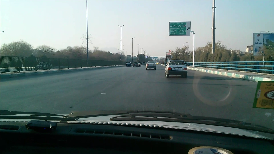
\includegraphics[width=65mm]{ev/eg11.png}
\hspace{-2mm}
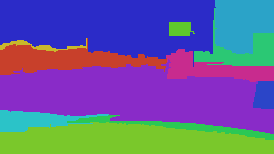
\includegraphics[width=65mm]{ev/eg1.png}

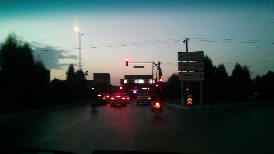
\includegraphics[width=65mm]{ev/eg22.png}
\hspace{-2mm}
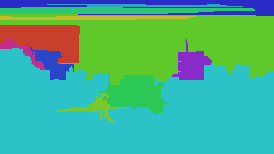
\includegraphics[width=65mm]{ev/eg2.png}


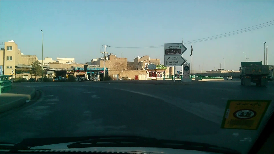
\includegraphics[width=65mm]{ev/eg33.png}
\hspace{-2mm}

\includegraphics[width=65mm]{ev/eg3.png}


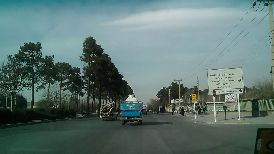
\includegraphics[width=65mm]{ev/eg44.png}
\hspace{-2mm}
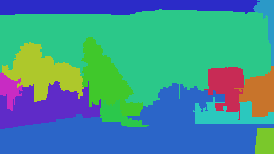
\includegraphics[width=65mm]{ev/eg4.png}


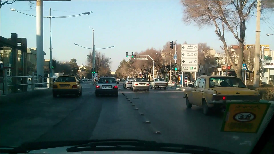
\includegraphics[width=65mm]{ev/eg55.png}
\hspace{-2mm}
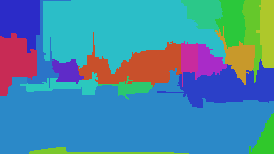
\includegraphics[width=65mm]{ev/eg5.png}


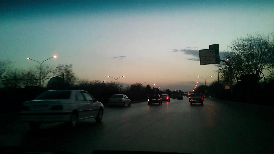
\includegraphics[width=65mm]{ev/eg66.png}
\hspace{-2mm}
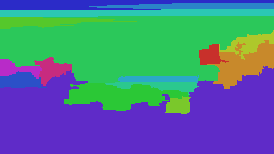
\includegraphics[width=65mm]{ev/eg6.png}

\caption[نواحی مثبت حاصل از فلان]
{نواحی مثبت حاصل از روش آقایون فلانی و فلانی مثلا}
\label{fig:evegbisreg}
\end{figure}


\FloatBarrier
\section{آزمایش هفتم: رد فلان روش}

لورم ایپسوم ( به انگلیسی \lr{lorem ipsum} ) متنی بی مفهوم است که تشکیل شده از کلمات معنی دار یا بی معنی کنار هم. کاربر با دیدن متن لورم ایپسوم تصور میکند متنی که در صفحه مشاهده میکند این متن واقعی و مربوط به توضیحات صفحه مورد نظر است واقعی است. حالا سوال اینجاست که این متن « لورم ایپسوم » به چه دردی میخورد و اساسا برای چه منظور و هدفی ساخته شده است؟ پیش از بوجود آمدن لورم ایپسوم ، طراحان وب سایت در پروژه های وب سایت و طراحان کرافیک در پروژه های طراحی کاتولوگ ، بروشورs ، پوستر و ... همواره با این مشکل مواجه بودند که صفحات پروژه خود را پیش از آنکه متن اصلی توسط کارفرما ارائه گردد و در صفحه مورد نظر قرار گیرد چگونه پر کنند؟؟ اکثر طراحان با نوشتن یک جمله مانند «این یک متن نمونه است» ویا «توضیحات در این بخش قرار خواهند گرفت» و کپی آن به تعداد زیاد یک یا چند پاراگراف متن میساختند که تمامی متن ها و کلمات ، جملات و پاراگراف ها تکراری بود و از این رو منظره خوبی برای بیننده نداشت و ضمنا به هیچ وجه واقعی به نظر نمیرسید تا بتواند شکل و شمایل تمام شده پروژه را نشان دهد. از این رو متنی ساخته شد که با دو کلمه ( به فارسی : لورم ایپسوم ) آغاز میشد وبا همین نام در بین طراحان وب و گرافیک شناخته و به سرعت محبوب شد. وب سایت های سازنده لورم ایپسوم میتوانند هر تعداد کلمه و پاراگراف که بخواهید به صوورت تکراری یا غیر تکراری برایتان بسازند و تحویلتان بدهند تا از آنها در پروژه هایتان استفاده کنید. ( لورم ایپسوم فارسی) متن های لورم ایپسوم را به زبان فارسی و علاوه بر زبان فارسی به انگلیسی ، عربی ، ترکی استانبولی و ... برایتان میسازد. زبان های دیگر نیز رفته رفته به بانک اطلاعاتی لورم ایسپوم فارسی اضافه خواهند شد.  


 \begin{figure}[!htb]
\centering   %%% not \center
\subfigure[تفاضل]{
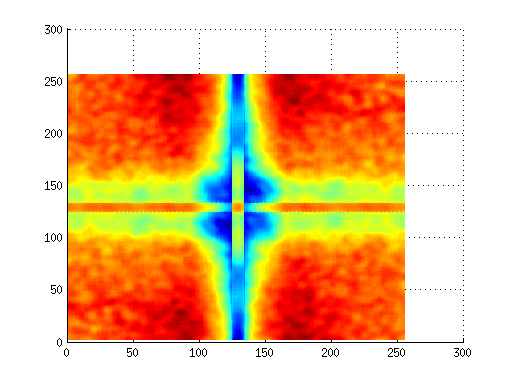
\includegraphics[width=7.5cm]{fft/diff-n.png}
\label{fig:fft-df}
}\hspace{-12mm}
\subfigure[تفاضلی دیگر]{
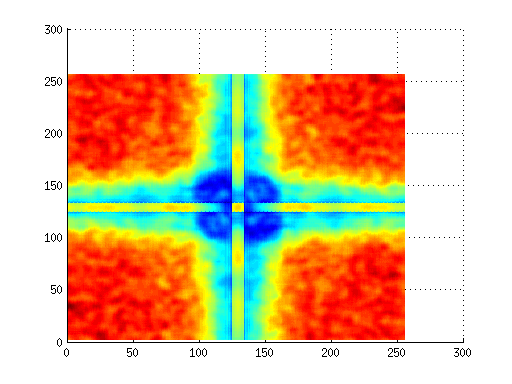
\includegraphics[width=7.5cm]{fft/diff-p.png}
\label{fig:fft-dp}
}
\caption[نمونه‌ی تفاضل در تشخیص درست]
{در  \subref{fig:fft-df} تفاضل با فلان و در \subref{fig:fft-dp} تفاضل با فلان آمده‌است.}
\label{fig:fft-diff}
\end{figure}
لورم ایپسوم ( به انگلیسی \lr{lorem ipsum} ) متنی بی مفهوم است که تشکیل شده از کلمات معنی دار یا بی معنی کنار هم. کاربر با دیدن متن لورم ایپسوم تصور میکند متنی که در صفحه مشاهده میکند این متن واقعی و مربوط به توضیحات صفحه مورد نظر است واقعی است. حالا سوال اینجاست که این متن « لورم ایپسوم » به چه دردی میخورد و اساسا برای چه منظور و هدفی ساخته شده است؟ پیش از بوجود آمدن لورم ایپسوم ، طراحان وب سایت در پروژه های وب سایت و طراحان کرافیک در پروژه های طراحی کاتولوگ ، بروشور ، پوستر و ... همواره با این مشکل مواجه بودند که صفحات پروژه خود را پیش از آنکه متن اصلی توسط کارفرما ارائه گردد و در صفحه مورد نظر قرار گیرد چگونه پر کنند؟؟ 

\FloatBarrier
\section{آزمایش هشتم: آزمایشی دیگر}
لورم ایپسوم ( به انگلیسی \lr{lorem ipsum} ) متنی بی مفهوم است که تشکیل شده از کلمات معنی دار یا بی معنی کنار هم. کاربر با دیدن متن لورم ایپسوم تصور میکند متنی که در صفحه مشاهده میکند این متن واقعی و مربوط به توضیحات صفحه مورد نظر است واقعی است. حالا سوال اینجاست که این متن « لورم ایپسوم » به چه دردی میخورد و اساسا برای چه منظور و هدفی ساخته شده است؟ پیش از بوجود آمدن لورم ایپسوم ، طراحان وب سایت در پروژه های وب سایت و طراحان کرافیک در پروژه های طراحی کاتولوگ ، بروشور ، پوستر و ... همواره با این مشکل مواجه بودند که صفحات پروژه خود را پیش از آنکه متن اصلی توسط کارفرما ارائه گردد و در صفحه مورد نظر قرار گیرد چگونه پر کنند؟؟ اکثر طراحان با نوشتن یک جمله مانند «این یک متن نمونه است» ویا «توضیحات در این بخش قرار خواهند گرفت» و کپی آن به تعداد زیاد یک یا چند پاراگراف متن میساختند که تمامی متن ها و کلمات ، جملات و پاراگراف ها تکراری بود و از این رو منظره خوبی برای بیننده نداشت و ضمنا به هیچ وجه واقعی به نظر نمیرسید تا بتواند شکل و شمایل تمام شده پروژه را نشان دهد. از این رو متنی ساخته شد که با دو کلمه ( به فارسی : لورم ایپسوم ) آغاز میشد وبا همین نام در بین طراحان وب و گرافیک شناخته و به سرعت محبوب شد. وب سایت های سازنده لورم ایپسوم میتوانند هر تعداد کلمه و پاراگراف که بخواهید به صوورت تکراری یا غیر تکراری برایتان بسازند و تحویلتان بدهند تا از آنها در پروژه هایتان استفاده کنید. ( لورم ایپسوم فارسی) متن های لورم ایپسوم را به زبان فارسی و علاوه بر زبان فارسی به انگلیسی ، عربی ، ترکی استانبولی و ... برایتان میسازد. زبان های دیگر نیز رفته رفته به بانک اطلاعاتی لورم ایسپوم فارسی اضافه خواهند شد.  


\FloatBarrier
\section{جمع‌بندی}

روش ارایه‌شده در تقسیم فضا به نواحی شامل تابلو به نسبت روش‌های پیشین عملکرد بهتری نشان داد .............


 
\cchapter{نتیجه‌گیری و پیشنهادات}
\label{chap:conclusion}
\pagebreak
لورم ایپسوم ( به انگلیسی \lr{lorem ipsum} ) متنی بی مفهوم است که تشکیل شده از کلمات معنی دار یا بی معنی کنار هم. کاربر با دیدن متن لورم ایپسوم تصور میکند متنی که در صفحه مشاهده میکند این متن واقعی و مربوط به توضیحات صفحه مورد نظر است واقعی است. حالا سوال اینجاست که این متن « لورم ایپسوم » به چه دردی میخورد و اساسا برای چه منظور و هدفی ساخته شده است؟ پیش از بوجود آمدن لورم ایپسوم ، طراحان وب سایت در پروژه های وب سایت و طراحان کرافیک در پروژه های طراحی کاتولوگ ، بروشور ، پوستر و ... همواره با این مشکل مواجه بودند که صفحات پروژه خود را پیش از آنکه متن اصلی توسط کارفرما ارائه گردد و در صفحه مورد نظر قرار گیرد چگونه پر کنند؟؟ اکثر طراحان با نوشتن یک جمله مانند «این یک متن نمونه است» ویا «توضیحات در این بخش قرار خواهند گرفت» و کپی آن به تعداد زیاد یک یا چند پاراگراف متن میساختند که تمامی متن ها و کلمات ، جملات و پاراگراف ها تکراری بود و از این رو منظره خوبی برای بیننده نداشت و ضمنا به هیچ وجه واقعی به نظر نمیرسید تا بتواند شکل و شمایل تمام شده پروژه را نشان دهد. از این رو متنی ساخته شد که با دو کلمه ( به فارسی : لورم ایپسوم ) آغاز میشد وبا همین نام در بین طراحان وب و گرافیک شناخته و به سرعت محبوب شد. وب سایت های سازنده لورم ایپسوم میتوانند هر تعداد کلمه و پاراگراف که بخواهید به صوورت تکراری یا غیر تکراری برایتان بسازند و تحویلتان بدهند تا از آنها در پروژه هایتان استفاده کنید. ( لورم ایپسوم فارسی) متن های لورم ایپسوم را به زبان فارسی و علاوه بر زبان فارسی به انگلیسی ، عربی ، ترکی استانبولی و ... برایتان میسازد. زبان های دیگر نیز رفته رفته به بانک اطلاعاتی لورم ایسپوم فارسی اضافه خواهند شد.  

لورم ایپسوم ( به انگلیسی \lr{lorem ipsum} ) متنی بی مفهوم است که تشکیل شده از کلمات معنی دار یا بی معنی کنار هم. کاربر با دیدن متن لورم ایپسوم تصور میکند متنی که در صفحه مشاهده میکند این متن واقعی و مربوط به توضیحات صفحه مورد نظر است واقعی است. حالا سوال اینجاست که این متن « لورم ایپسوم » به چه دردی میخورد و اساسا برای چه منظور و هدفی ساخته شده است؟ پیش از بوجود آمدن لورم ایپسوم ، طراحان وب سایت در پروژه های وب سایت و طراحان کرافیک در پروژه های طراحی کاتولوگ ، بروشور ، پوستر و ... همواره با این مشکل مواجه بودند که صفحات پروژه خود را پیش از آنکه متن اصلی توسط کارفرما ارائه گردد و در صفحه مورد نظر قرار گیرد چگونه پر کنند؟؟ اکثر طراحان با نوشتن یک جمله مانند «این یک متن نمونه است» ویا «توضیحات در این بخش قرار خواهند گرفت» و کپی آن به تعداد زیاد یک یا چند پاراگراف متن میساختند که تمامی متن ها و کلمات ، جملات و پاراگراف ها تکراری بود و از این رو منظره خوبی برای بیننده نداشت و ضمنا به هیچ وجه واقعی به نظر نمیرسید تا بتواند شکل و شمایل تمام شده پروژه را نشان دهد. از این رو متنی ساخته شد که با دو کلمه ( به فارسی : لورم ایپسوم ) آغاز میشد وبا همین نام در بین طراحان وب و گرافیک شناخته و به سرعت محبوب شد. وب سایت های سازنده لورم ایپسوم میتوانند هر تعداد کلمه و پاراگراف که بخواهید به صوورت تکراری یا غیر تکراری برایتان بسازند و تحویلتان بدهند تا از آنها در پروژه هایتان استفاده کنید. ( لورم ایپسوم فارسی) متن های لورم ایپسوم را به زبان فارسی و علاوه بر زبان فارسی به انگلیسی ، عربی ، ترکی استانبولی و ... برایتان میسازد. زبان های دیگر نیز رفته رفته به بانک اطلاعاتی لورم ایسپوم فارسی اضافه خواهند شد.  

لورم ایپسوم ( به انگلیسی \lr{lorem ipsum} ) متنی بی مفهوم است که تشکیل شده از کلمات معنی دار یا بی معنی کنار هم. کاربر با دیدن متن لورم ایپسوم تصور میکند متنی که در صفحه مشاهده میکند این متن واقعی و مربوط به توضیحات صفحه مورد نظر است واقعی است. حالا سوال اینجاست که این متن « لورم ایپسوم » به چه دردی میخورد و اساسا برای چه منظور و هدفی ساخته شده است؟ پیش از بوجود آمدن لورم ایپسوم ، طراحان وب سایت در پروژه های وب سایت و طراحان کرافیک در پروژه های طراحی کاتولوگ ، بروشور ، پوستر و ... همواره با این مشکل مواجه بودند که صفحات پروژه خود را پیش از آنکه متن اصلی توسط کارفرما ارائه گردد و در صفحه مورد نظر قرار گیرد چگونه پر کنند؟؟ اکثر طراحان با نوشتن یک جمله مانند «این یک متن نمونه است» ویا «توضیحات در این بخش قرار خواهند گرفت» و کپی آن به تعداد زیاد یک یا چند پاراگراف متن میساختند که تمامی متن ها و کلمات ، جملات و پاراگراف ها تکراری بود و از این رو منظره خوبی برای بیننده نداشت و ضمنا به هیچ وجه واقعی به نظر نمیرسید تا بتواند شکل و شمایل تمام شده پروژه را نشان دهد. از این رو متنی ساخته شد که با دو کلمه ( به فارسی : لورم ایپسوم ) آغاز میشد وبا همین نام در بین طراحان وب و گرافیک شناخته و به سرعت محبوب شد. وب سایت های سازنده لورم ایپسوم میتوانند هر تعداد کلمه و پاراگراف که بخواهید به صوورت تکراری یا غیر تکراری برایتان بسازند و تحویلتان بدهند تا از آنها در پروژه هایتان استفاده کنید. ( لورم ایپسوم فارسی) متن های لورم ایپسوم را به زبان فارسی و علاوه بر زبان فارسی به انگلیسی ، عربی ، ترکی استانبولی و ... برایتان میسازد. زبان های دیگر نیز رفته رفته به بانک اطلاعاتی لورم ایسپوم فارسی اضافه خواهند شد.  

\section{پیشنهادات}
به طور کلی پیشنهادها برای پژوهش‌های آتی به این صورت است:

لورم ایپسوم ( به انگلیسی \lr{lorem ipsum} ) متنی بی مفهوم است که تشکیل شده از کلمات معنی دار یا بی معنی کنار هم. کاربر با دیدن متن لورم ایپسوم تصور میکند متنی که در صفحه مشاهده میکند این متن واقعی و مربوط به توضیحات صفحه مورد نظر است واقعی است. حالا سوال اینجاست که این متن « لورم ایپسوم » به چه دردی میخورد و اساسا برای چه منظور و هدفی ساخته شده است؟ پیش از بوجود آمدن لورم ایپسوم ، طراحان وب سایت در پروژه های وب سایت و طراحان کرافیک در پروژه های طراحی کاتولوگ ، بروشور ، پوستر و ... همواره با این مشکل مواجه بودند که صفحات پروژه خود را پیش از آنکه متن اصلی توسط کارفرما ارائه گردد و در صفحه مورد نظر قرار گیرد چگونه پر کنند؟؟ اکثر طراحان با نوشتن یک جمله مانند «این یک متن نمونه است» ویا «توضیحات در این بخش قرار خواهند گرفت» و کپی آن به تعداد زیاد یک یا چند پاراگراف متن میساختند که تمامی متن ها و کلمات ، جملات و پاراگراف ها تکراری بود و از این رو منظره خوبی برای بیننده نداشت و ضمنا به هیچ وجه واقعی به نظر نمیرسید تا بتواند شکل و شمایل تمام شده پروژه را نشان دهد. از این رو متنی ساخته شد که با دو کلمه ( به فارسی : لورم ایپسوم ) آغاز میشد وبا همین نام در بین طراحان وب و گرافیک شناخته و به سرعت محبوب شد. وب سایت های سازنده لورم ایپسوم میتوانند هر تعداد کلمه و پاراگراف که بخواهید به صوورت تکراری یا غیر تکراری برایتان بسازند و تحویلتان بدهند تا از آنها در پروژه هایتان استفاده کنید. ( لورم ایپسوم فارسی) متن های لورم ایپسوم را به زبان فارسی و علاوه بر زبان فارسی به انگلیسی ، عربی ، ترکی استانبولی و ... برایتان میسازد. زبان های دیگر نیز رفته رفته به بانک اطلاعاتی لورم ایسپوم فارسی اضافه خواهند شد.  



\newpage
%\begin{latin}
\pagestyle{plain}
{
\onehalfspacing
\bibliographystyle{ieeetr-fa}%{chicago-fa}%{plainnat-fa}%
\bibliography{Thesis}
}
%\end{latin}

\newpage


\appendix
\renewcommand{\chaptername}{پیوست}
\pagebreak
%\addappheadtotoc
\addcontentsline{toc}{chapter}{‌پیوست‌ها}
\addtocontents{toc}{\protect\setcounter{tocdepth}{-1}}

\cchapter{نمونه‌هایی از دادگان}
%\setcounter{chapter}{1}
\newpage

\pagenumbering{arabic}\renewcommand{\thepage}{\arabic{chapter}-\arabic{page}}
%\addcontentsline{toc}{section}{‌پیوست‌ آ - نمونه‌هایی از دادگان}


\begin{figure}[ht]
\floatpagestyle{plain}
\centering     %%% not \center

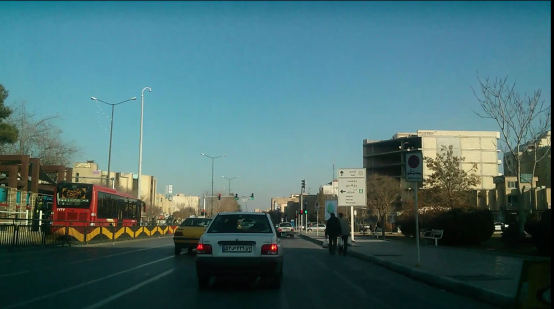
\includegraphics[width=120mm]{x/x1.png}
%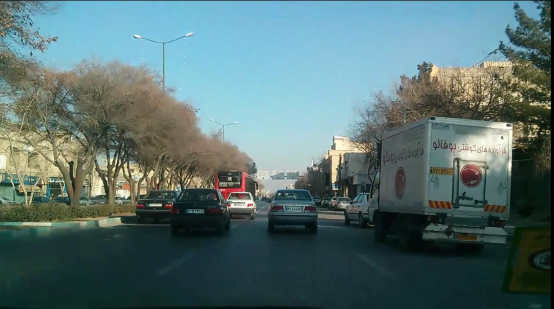
\includegraphics[width=60mm]{x/x2.png}

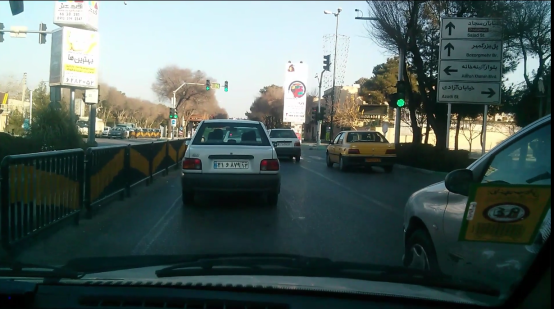
\includegraphics[width=120mm]{x/x3.png}
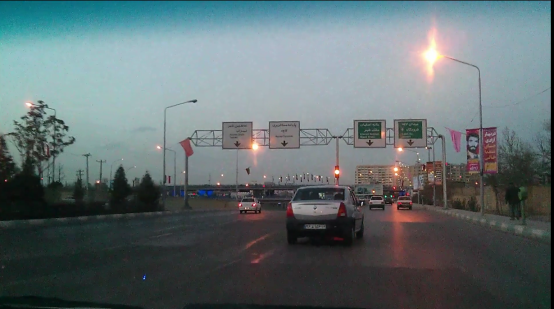
\includegraphics[width=120mm]{x/x4.png}

%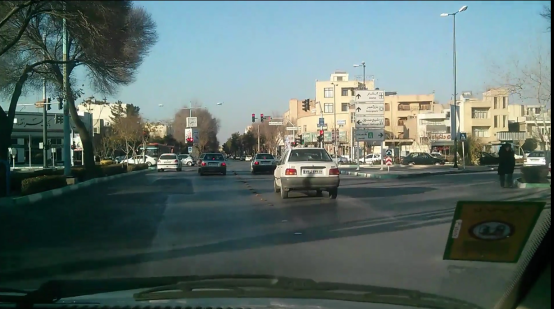
\includegraphics[width=60mm]{x/x5.png}
%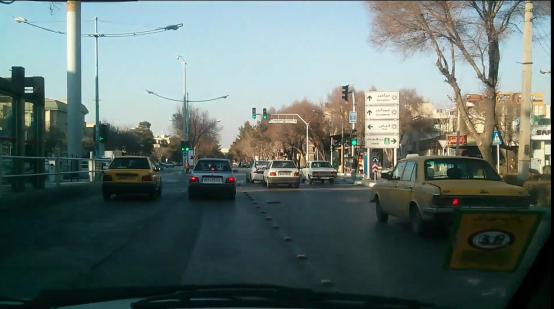
\includegraphics[width=60mm]{x/x6.png}

%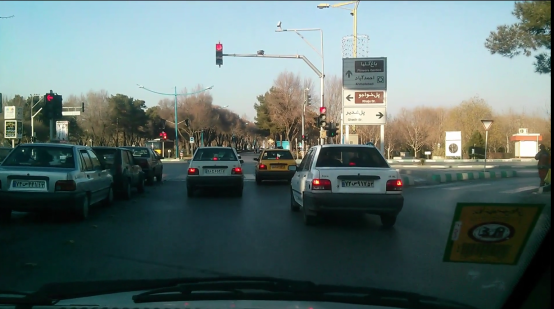
\includegraphics[width=60mm]{x/x7.png}
%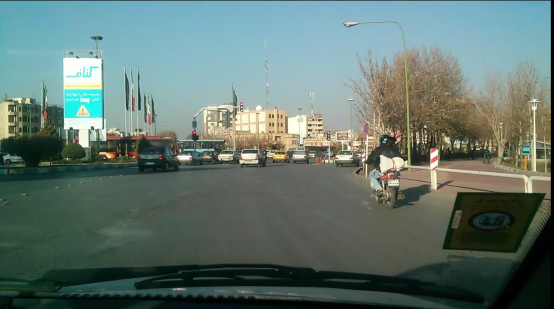
\includegraphics[width=60mm]{x/x8.png}

%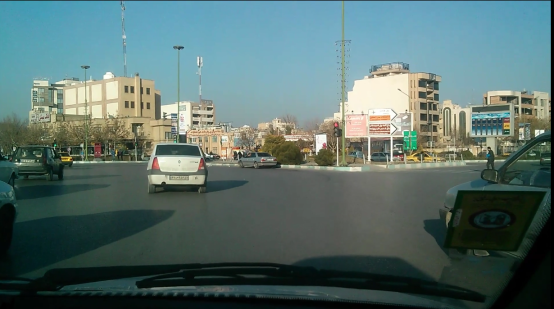
\includegraphics[width=60mm]{x/x9.png}
%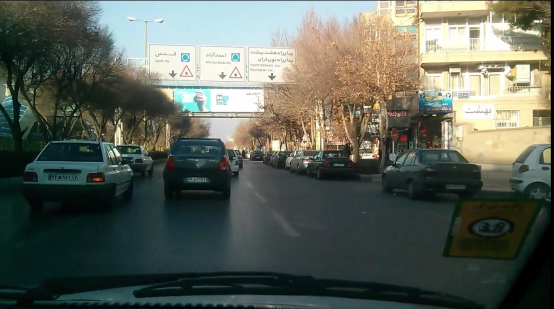
\includegraphics[width=60mm]{x/x10.png}

%\includegraphics[width=60mm]{x/x11.png}
%\includegraphics[width=60mm]{x/x12.png}

\caption{نمونه دادگان}
\label{fig:append1}
\end{figure}


\vspace{-1cm}
\begin{figure}[ht]
\floatpagestyle{plain}
\centering     %%% not \center
\includegraphics[width=120mm]{x/x5.png}
\includegraphics[width=120mm]{x/x7.png}
\includegraphics[width=120mm]{x/x8.png}

\caption{نمونه دادگان}
\label{fig:append2}
\end{figure}

\vspace{-1cm}
\begin{figure}[ht]
\floatpagestyle{plain}
\centering     %%% not \center
\includegraphics[width=120mm]{x/x13.png}
\includegraphics[width=120mm]{x/x14.png}
\includegraphics[width=120mm]{x/x16.png}

\caption{نمونه دادگان}
\label{fig:append3}
\end{figure}


\vspace{-1cm}
\begin{figure}[ht]
\floatpagestyle{plain}
\centering     %%% not \center
\includegraphics[width=120mm]{x/x22.png}
\includegraphics[width=120mm]{x/x25.png}
\includegraphics[width=120mm]{x/x24.png}

\caption{نمونه دادگان}
\label{fig:append4}
\end{figure}

\vspace{-1cm}
\begin{figure}[ht]
\floatpagestyle{plain}
\centering     %%% not \center
\includegraphics[width=120mm]{x/x37.png}
\includegraphics[width=120mm]{x/x38.png}
\includegraphics[width=120mm]{x/x40.png}

\caption{نمونه دادگان}
\label{fig:append5}
\end{figure}

%\end{latin}
%\end{spacing}

\begin{latin}
\latinfirstPage
\end{latin}
\end{document} 
